\documentclass[conference]{IEEEtran}
\IEEEoverridecommandlockouts
% The preceding line is only needed to identify funding in the first footnote. If that is unneeded, please comment it out.
\usepackage{cite}
\usepackage{amsmath,amssymb,amsfonts}
\usepackage{algorithmic}
\usepackage{graphicx}
\usepackage{textcomp}
\usepackage{xcolor}
\usepackage{ctex}
\usepackage{fontspec}
\usepackage{listings}
\usepackage{pxfonts}
% The following code is for matlab language
\lstset{
    columns=fixed,     
    basicstyle = \tt,           % 基本样式 + 小号字体  
    frame=none,     % 不显示背景边框
    breaklines = true,                  % 代码过长则换行
    backgroundcolor=\color[RGB]{245,245,244},  % 设定背景颜色
    keywordstyle=\color[RGB]{40,40,255},         % 设定关键字颜色
    commentstyle=\it\color[RGB]{0,96,96},         % 设置代码注释的格式
    stringstyle=\rmfamily\slshape\color[RGB]{128,0,0},   % 设置字符串格式
    showstringspaces=false,   % 不显示字符串中的空格
    language=python,             % 设置语言
    extendedchars=false,
    tabsize=4,
    upquote=true,
}

\def\BibTeX{{\rm B\kern-.05em{\sc i\kern-.025em b}\kern-.08em
    T\kern-.1667em\lower.7ex\hbox{E}\kern-.125emX}}
\begin{document}

\title{傅立叶变换光谱测量技术实验报告}

\author{
    \IEEEauthorblockN{
        黄润华}
        \IEEEauthorblockA{
            \textit{Ocean University of China} \\
            \textit{email@noreply.com}
    \and
    \IEEEauthorblockN{
        杨超}
        \IEEEauthorblockA{
            \textit{Ocean University of China} \\
            \textit{email@somewhere.com}
        }
    }
}

\maketitle

\begin{abstract}
    本实验报告为傅立叶变换光谱测量技术第三次实验报告,本报告采用Python仿真对干涉波形补零与加窗环境下的傅里叶变换光谱测量系统的光谱测量曲线。中心波长选择632.8nm。
\end{abstract}

\begin{IEEEkeywords}
    Optical spectrum, python, fft
\end{IEEEkeywords}

\section{实验目的}
\begin{itemize}
    \item 思考干涉图补零对傅里叶变换光谱测量曲线的影响
    \item 思考干涉图加不同窗后补零对傅里叶变换光谱测量曲线的影响
    \item 学习利用Python仿真不同影响条件下光谱测量曲线。
\end{itemize}

\section{实验原理}

\subsection{分辨率和分辨能力}
光谱仪的光谱分辨率是其定性区分彼此非常接近的两个光谱峰的能力的量度。 通常,光谱分辨率由仪器线形状(ILS)的半峰全宽(FWHM)表示,光谱仪的输出光谱具有纯单色输入辐射。

光谱分辨率R由下式定义
\begin{align}
    R = \frac{\sigma_{max}}{\delta \sigma}
\end{align}
其中$\sigma_{max}$是光谱仪设计运行的最大波数。

\subsubsection{分辨率与最大OPD之间的关系}
根据公式
\begin{align}
    B_{c}(\sigma)=B_{r e L}(\sigma)+i B_{i o L}(\sigma)=\int_{-\infty}^{\infty} I(x) \operatorname{rect}(x) e^{-i 2 \pi a x} d x \\
    \begin{cases}{c}
        B(\sigma)=2 \mid \int_{-\infty}^{+\infty} I(x) \operatorname{rect}(x) e^{-2 \pi a x} d x \\
        \phi(\sigma)=\arctan \left[\frac{B_{i o L}(\sigma)}{B_{r e L}(\sigma)}\right]
    \end{cases} \quad(\sigma \geq 0)
\end{align}
其中矩形函数定义为
\begin{align*}
    \operatorname{rect}(x)=\begin{cases}
        1 & |x|<L \\
        0 & |x|>L
        \end{cases}
\end{align*}
因此,理论上 FTS 的光谱分辨率取决于可移动镜的扫描范围
\begin{align}
    B_{e}(\sigma)=\begin{cases}{ll}
        B(\sigma) / 2 & (\sigma \geq 0) \\
        B(-\sigma) / 2 & (\sigma \leq 0)
        \end{cases}
\end{align}
理论上,完美单色线的干涉图可以用来描述
\begin{align}
    I(x) = 2cos(2\pi \sigma_0 x)
\end{align}
将此表达式替换为方程$B(\sigma)$、$\phi(\sigma)$,考虑到实际上$\sigma > 0$,可以得到ILS $B(\sigma)$的表达式:
\begin{align}
        B_{I I S}(\sigma)
        &=2 L\frac{\sin \left[2 \pi\left(\sigma_{0}+\sigma\right) L\right]}{2 \pi\left(\sigma_{0}+\sigma\right) L}+\frac{\sin \left[2 \pi\left(\sigma_{0}-\sigma\right) L\right]}{2 \pi\left(\sigma_{0}-\sigma\right) L} \\
        & \approx 2 L \times \frac{\sin \left[2 \pi\left(\sigma_{0}-\sigma\right) L\right]}{2 \pi\left(\sigma_{0}-\sigma\right) L}  \\
        & =2 L \sin c\left[2 \pi\left(\sigma_{0}-\sigma\right) L\right]
\end{align}
如图\ref{pic8}所示,光谱从一条线($\delta$ 函数)扩展到 $sin c$ 函数形状(仪器线形)。
\begin{align}
    (\delta \sigma)_{linewidth} = \frac{1.21}{2L}
\end{align}

\begin{figure}[htbp]
    \centerline{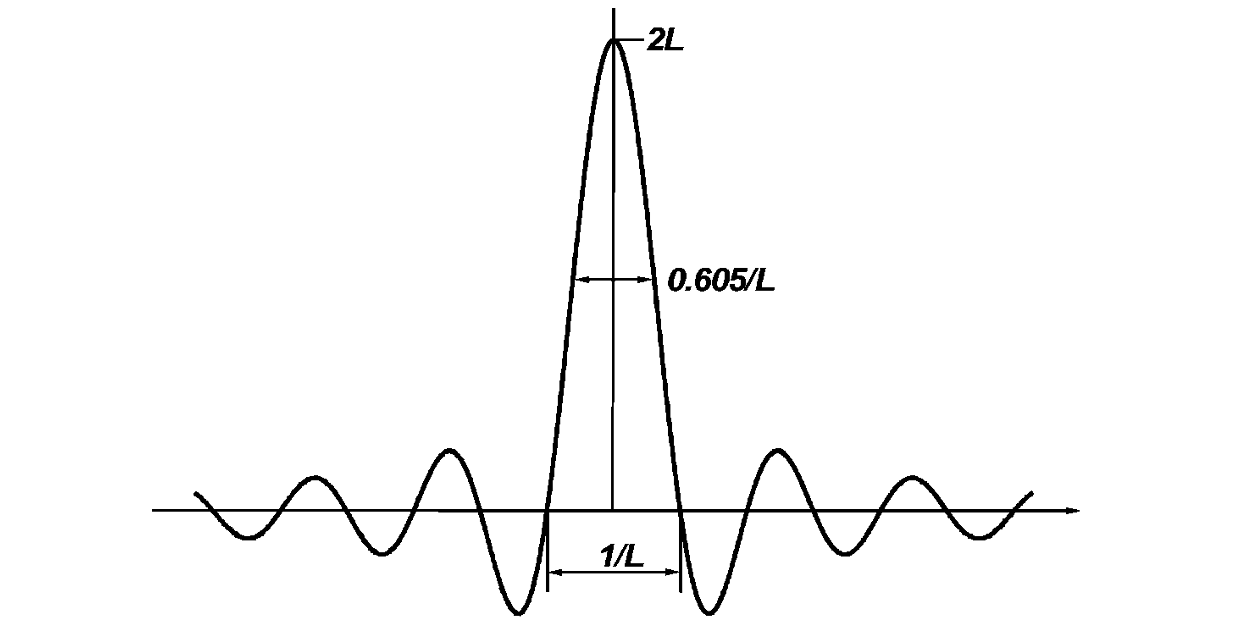
\includegraphics[width=0.5\textwidth]{pic8.png}}
    \caption{$B_{I I S}(\sigma)$}
    \label{pic8}
\end{figure}

\subsubsection{分离共振}
分辨率可以通过分离图\ref{pic9}所示光谱中相同强度(或共振)的两条单色线(波数和)来描述。
如果两个线峰值之间的下降幅度大于线峰值的 20\%,则可以声称解决了两个共振,此时
\begin{align}
    (\delta \sigma)_{separation} = \frac{1.46}{2L}
\end{align}

\begin{figure}[htbp]
    \centerline{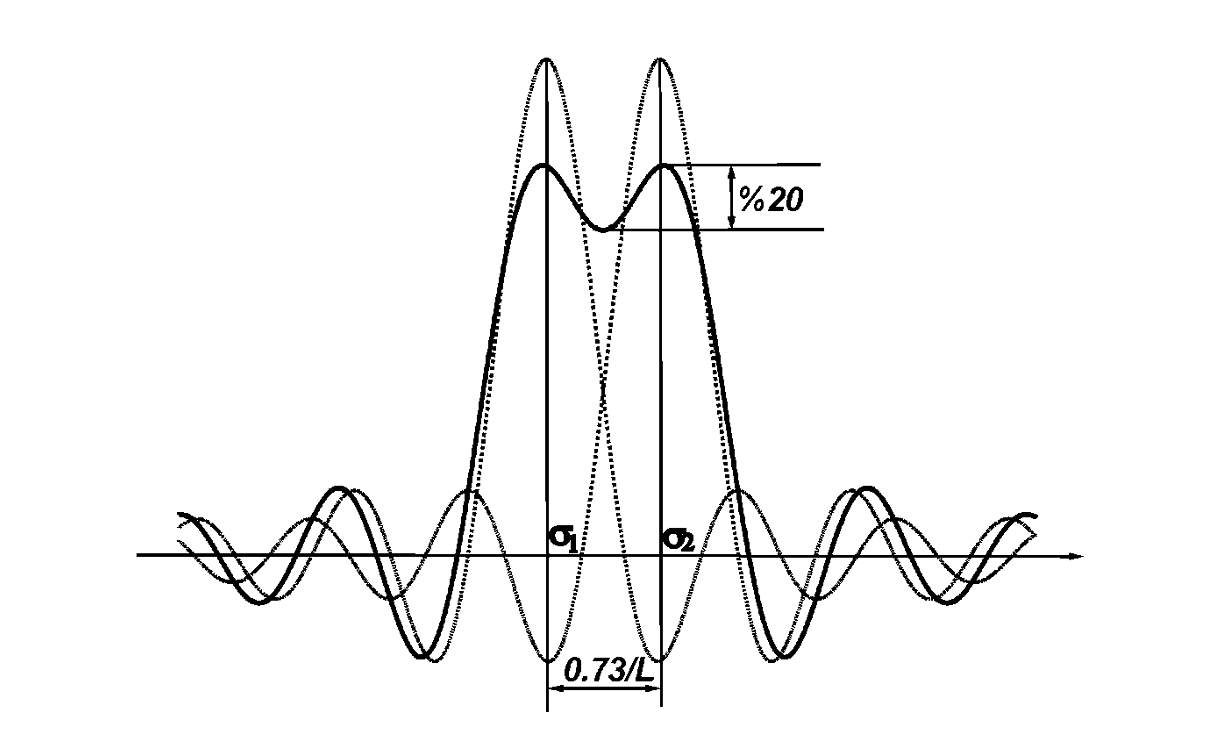
\includegraphics[width=0.5\textwidth]{pic9.png}}
    \caption{分离共振解析结果}
    \label{pic9}
\end{figure}

\subsubsection{瑞利准则}
瑞利准则分离两个 ILS 的峰值,使得一个共振的最大值落在另一个共振的零点处,因此,仪器线形状决定的分辨率是
\begin{align}
    \delta \sigma = \frac{1}{2L}
\end{align} 

\subsection{分辨率与发散角度之间的关系}
图\ref{pic10}是迈克尔逊干涉仪的等效图,根据图\ref{pic10}与图\ref{pic11}可以计算出OPD与夹角$\theta$之间的关系
\begin{align}
    O P D=2 \times \frac{x / 2}{\cos \theta}-x \tan \theta \sin \theta=x \cos \theta
\end{align}

\begin{figure}[htbp]
    \centerline{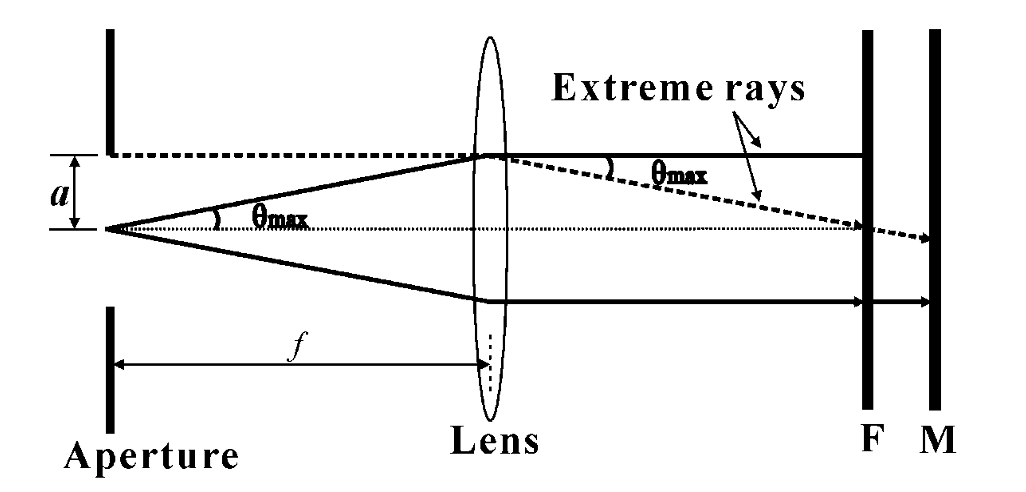
\includegraphics[width=0.5\textwidth]{pic10.png}}
    \caption{迈克尔逊干涉仪的等效图}
    \label{pic10}
\end{figure}

\begin{figure}[htbp]
    \centerline{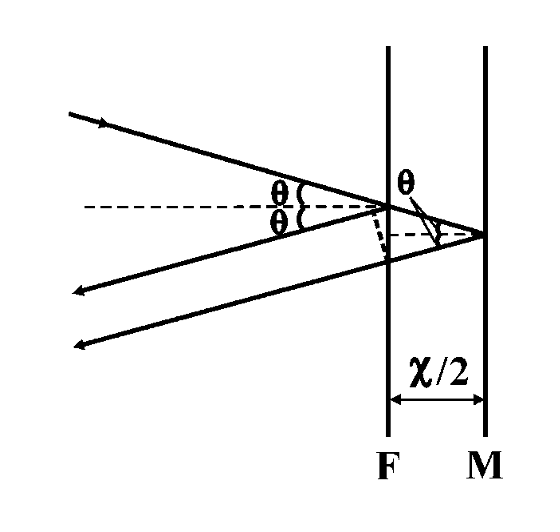
\includegraphics[width=0.5\textwidth]{pic11.png}}
    \caption{迈克尔逊干涉仪接收端放大图}
    \label{pic11}
\end{figure}
我们可以得到扩展源的归一化干涉图,对着一个立体角$\Omega_{max}$是
\begin{align*}
    I\left(x, \Omega_{\max }\right)=\frac{1}{\Omega_{\max }}\int_{0}^{\infty} B(\sigma) \int_{0}^{\Omega_{\operatorname{mix}}} \cos (2 \pi \sigma x \cos \theta) d \Omega d \sigma
\end{align*}
根据立体角的公式,上述式子可以化简为
\begin{align*}
    I\left(x, \Omega_{\max }\right)=\int_{0}^{\infty} B(\sigma) sinc \frac{\Omega_{\max } \sigma x }{2}  &\cos [2 \pi \sigma x\\
    & \;\;\;\;\;\;\;\;\;- \frac{\Omega_{\max } \sigma x }{2}] d \sigma
\end{align*}
对于单色光源其满足
\begin{align*}
    B(\sigma) = \delta(\sigma-\sigma_0)
\end{align*}
其仪器线轮廓可以写为
\begin{align*}
    \begin{cases}
        B_{D i v-1 L S}(\sigma)=[\pi /(\sigma_{0} \Omega_{\max })] \operatorname{rect}(\sigma_{1}, \sigma_{2})\\ \;\;\;\;\;\;\;\;\;\;\;\;\;\;\;\;\;\;\;\;\;\;\;\;\;\;\;\;\;\;\;\;+[\pi /(\sigma_{0} \Omega_{\max })] \operatorname{rect}(-\sigma_{2},-\sigma_{1}) \\
        \sigma_{2}=\sigma_{0}-\sigma_{0} \Omega_{\max } / 2 \pi \\
        \sigma_{1}=\sigma_{0}
    \end{cases}
\end{align*}
于是可以得到
\begin{align}
    &B_{D i v-1 L S}(\sigma)=\left[\pi /\left(\sigma_{0} \Omega_{\max }\right) \operatorname{lrect}\left(\sigma_{1}, \sigma_{2}\right)\right. \\
    &\bar{\sigma}=\sigma_{0}\left[1-\left(\Omega_{\max } / 4 \pi\right)\right]
\end{align}
总的波数差或分辨率是
\begin{align*}
    \delta \sigma = \frac{\sigma_0\Omega_{max}}{2\pi}
\end{align*}
考虑到可移动镜的扫描长度有限,实际 FTS 的 ILS 应该是
\begin{align}
    B_{I L S}(\sigma)=B_{D i v-I L S}(\sigma) * 2 L \sin c[2 \pi \sigma L]
\end{align}
其中$L$是可移动镜的最大位移,$*$是卷积算子。
图\ref{pic11}中两个极端射线的OPD之间的差异公式如下:
\begin{align*}
    \Delta O P D=2 L-2 L \cos \theta_{\max } \approx L \theta_{\max }^{2}=L \frac{a^{2}}{ f^{2}}
\end{align*}
其中$a$是入口孔径的半径,$f$是准直器的焦距。当$\Delta OPD$等于$\lambda/2$时,两条光线异相,它们之
间会发生破坏性叠加。对于宽带辐射输入,存在的最短波长决定了 FTS 的$\Delta OPD$的最大有效值, 如下式所示:
\begin{align}
    \Delta OPD \leq \frac{\lambda_{min}}{2} = \frac{1}{2\sigma_{max}}
\end{align}
我们可以得到 $a$的值应满足以下不等式, 以获得大于$R$的分辨率:
\begin{align}
    a \leq \frac{f}{\sqrt{R}}
\end{align}


\subsection{傅里叶变换光谱仪的优点}
与色散光谱仪相比,FTS具有许多广泛宣传的优点。然而,只有吞吐量(Jacquinot)和多路复用(Felgett)优势是FTS操作原理所固有的,而不是特定的工程设计。
\subsubsection{吞吐量或Jacquinot优势} 吞吐量优势是FTS可以具有大的圆形入口孔,其面积比分散光谱仪中的狭缝的面积大得多,以获得相同的分辨率。吞吐量 定义为 ,其中 是限制孔径的面积,并且是图\ref{pic12}中所示的准直或聚焦光学器件所对应的立体角。

FTS的最大吞吐量由下式给出
\begin{align}
    T_{FTS} = A\Omega_s = \frac{\pi}{R}A_{mirror}
\end{align}
其中$A_{mirror}$是镜子的投影面积。

\begin{figure}[htbp]
    \centerline{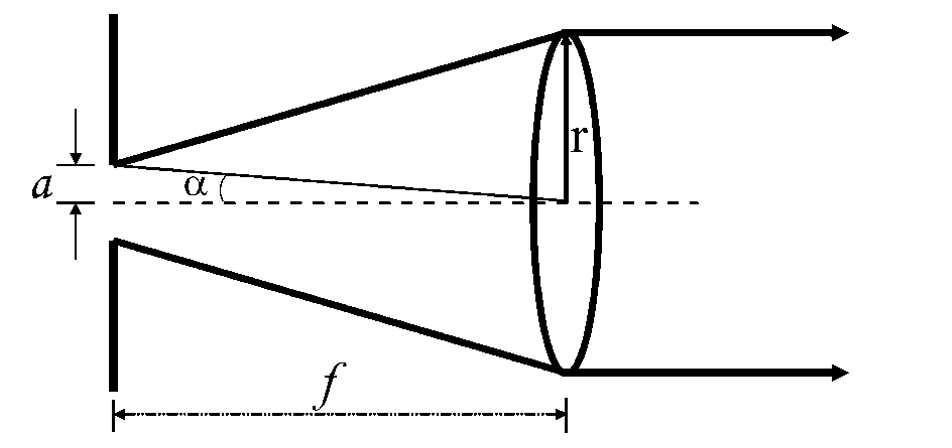
\includegraphics[width=0.5\textwidth]{pic12.png}}
    \caption{孔径和立体角的关系图}
    \label{pic12}
\end{figure}

对于光栅光谱仪,实现分辨率R的能量吞吐量受其狭缝区域和准直光学系统的限制,并由下式给出:
\begin{align}
    T_{grating} = \frac{l}{f_gR}A_{grating}
\end{align}
其中$f_g$是准直光学系统的焦距,$l$是狭缝的高度,$A_{grating}$是光栅的投影面积。对于光栅光谱仪,$\frac{l}{f_gR}$小于1/20。

因此,对于相同的分辨率和类似的仪器尺寸,FTS比光栅光谱仪具有高60倍的能量收集能力。 因此,Jacquinot的优势使得FTS更适合于弱信号测量,其中检测器噪声占主导地位,频谱信噪比(SNR)与吞吐量成比例地增加。

\subsubsection{Multiplex或Felgett的优势} 
多路复用的优点是FTS在扫描周期内同时观察来自给定频谱的整个范围的所有频谱信息。因此,通过使用FTS和使用单色仪可获得的SNR的比率:
\begin{align}
    \frac{SNR^S_{FTS}}{SNR_{monochromator}} = N^{\frac{1}{2}}
\end{align}
FTS的多重优势仅存在于红外和远红外信号的测量中,并且在可见 - 紫外信号的检测中丢失,因为在红外检测中,与信号电平无关的检测器噪声占主导地位。 量子噪声在可见光 - 紫外信号检测中占主导地位。
\subsubsection{Connes的优势}
FTS的波数范围来自He-Ne激光条纹,其作为每次扫描中采样位置的内部参考。 这种激光的波数非常准确,并且非常稳定。 因此,干涉仪的波数校准更精确,并且具有比分散仪器的校准好得多的长期稳定性.


\section{实验内容}
\begin{itemize}
    \item[1.] 仿真对于干涉图补零后的傅里叶变换光谱测量曲线,观察其变化。
    \item[2.] 仿真对于干涉图加窗函数并补零后的傅里叶变换光谱测量曲线,观察期变化。(以632.8nm的He-Ne激光为例,光程差采样间隔为79.1nm)
\end{itemize}

\begin{figure*}[htbp]
	\centerline{
		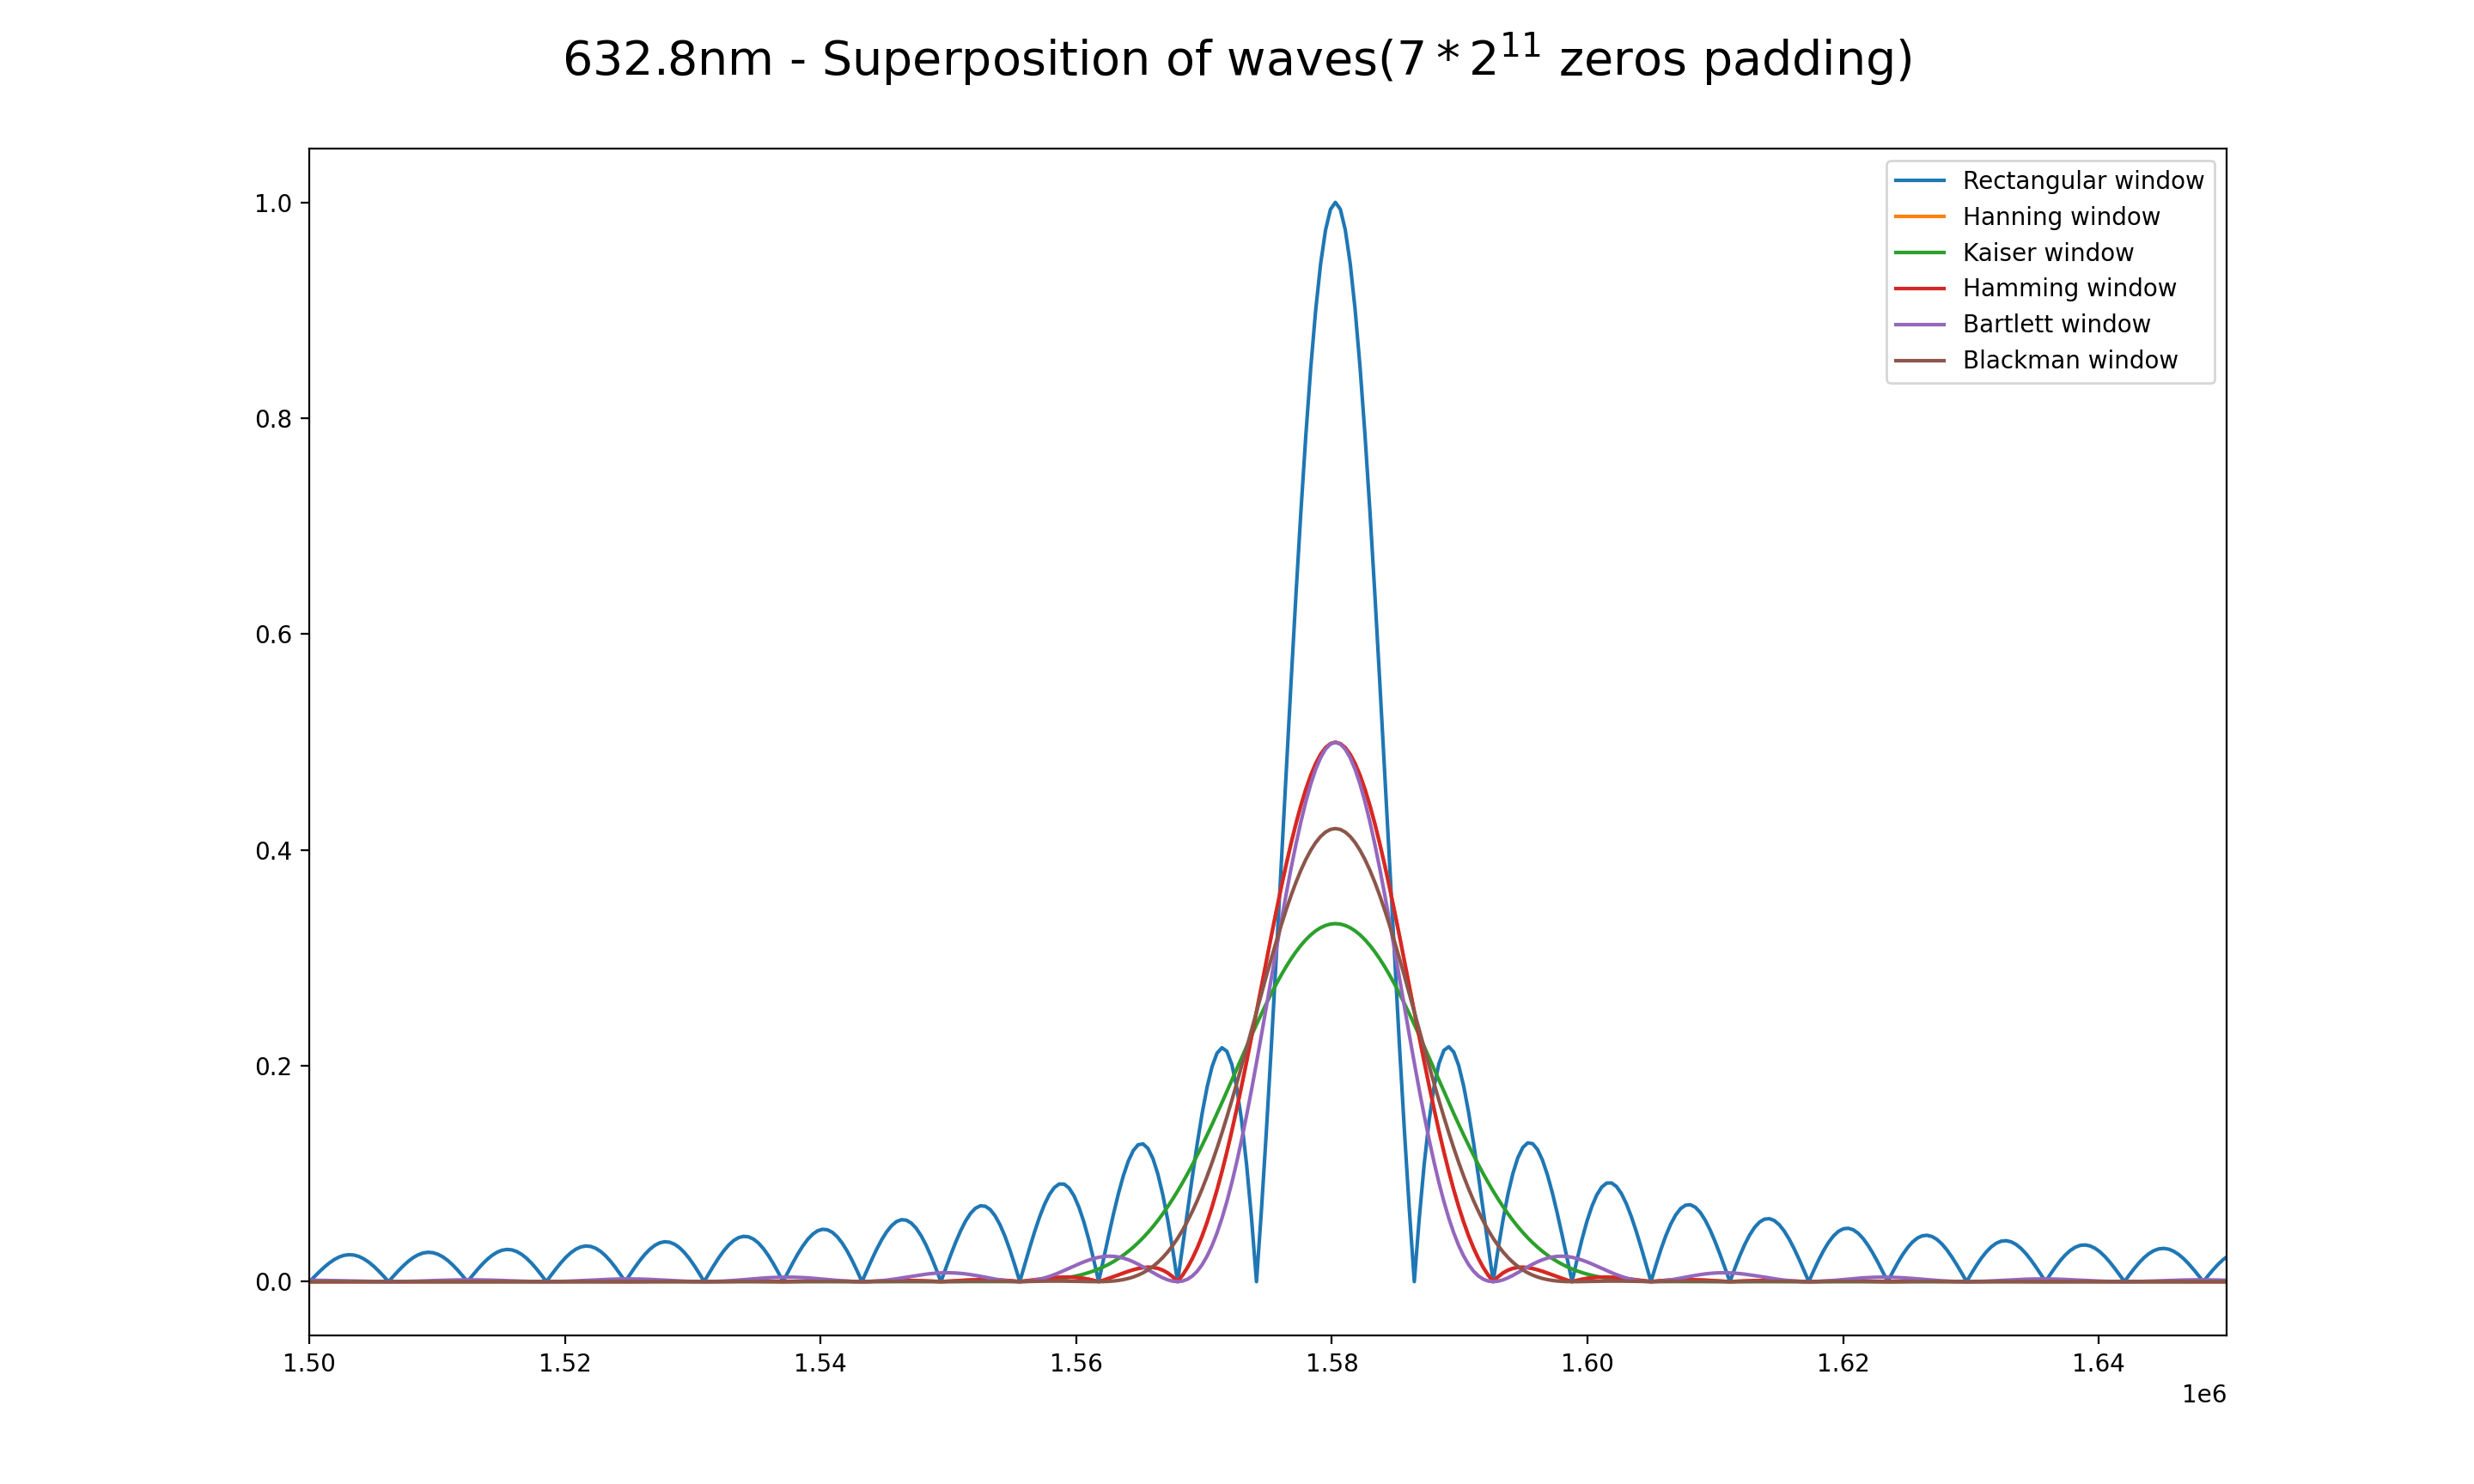
\includegraphics[width=22cm]{pic7.png} 	
	}
	\caption{加窗后与未加窗的光谱测量曲线的比较}
	\label{pic7}
\end{figure*}

\section{实验结果}

\subsection{加窗实验结果}
图片\ref{pic7}显示了加窗后与未加窗的光谱测量曲线的比较结果。加窗前与加窗后干涉图补零的个数均为$7\times2^{11}$个。更详细具体的加窗图片如图\ref{pic13}至\ref{pic17}所示,每张图片显示了对干涉图加特殊窗后与对干涉图加矩形窗(未加窗)的比较结果。图片左侧显示了干涉图加窗的波形,右侧图片为光谱测量曲线的波形,右侧黄色部分的线表示光谱测量曲线的半波全宽。
\begin{figure}[htbp]
    \centerline{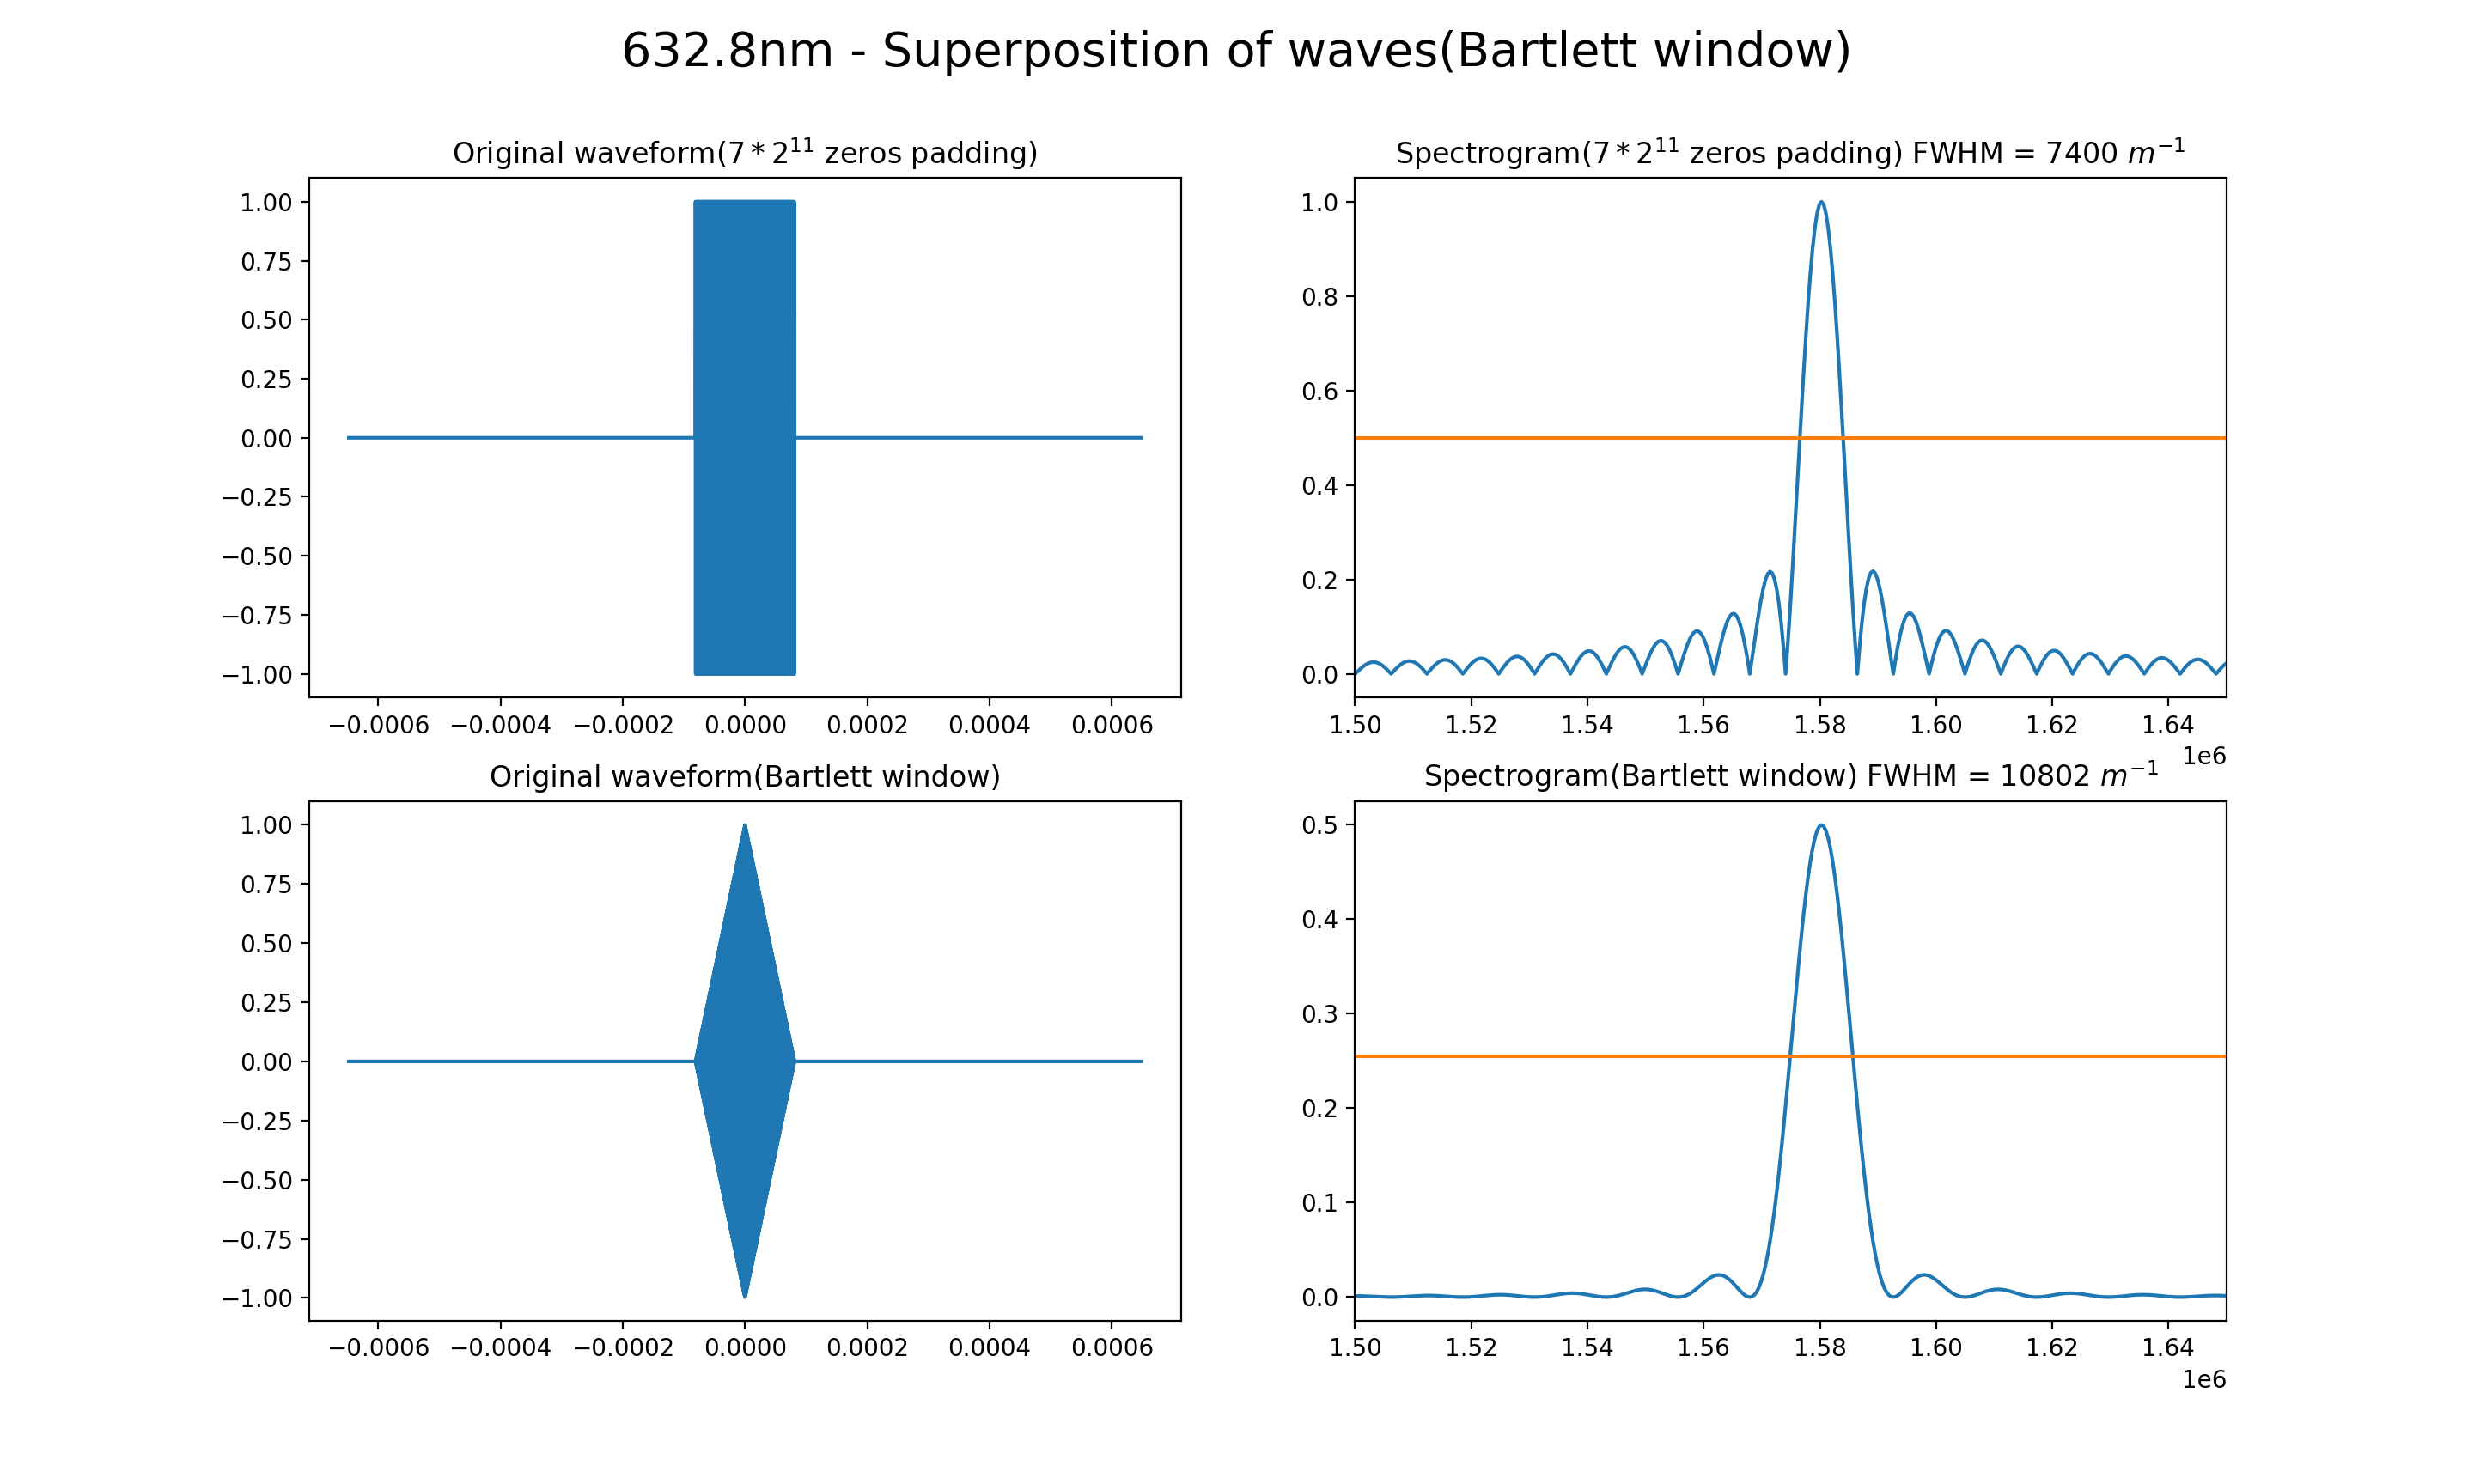
\includegraphics[width=0.5\textwidth]{Bartlett.png}}
    \caption{对干涉图分别加Bartlett窗与矩形窗的比较,图片左侧显示了干涉图加窗的波形,右侧图片为光谱测量曲线的波形,右侧黄色部分的线表示光谱测量曲线的半波全宽}
    \label{pic13}
\end{figure}

\begin{figure}[htbp]
    \centerline{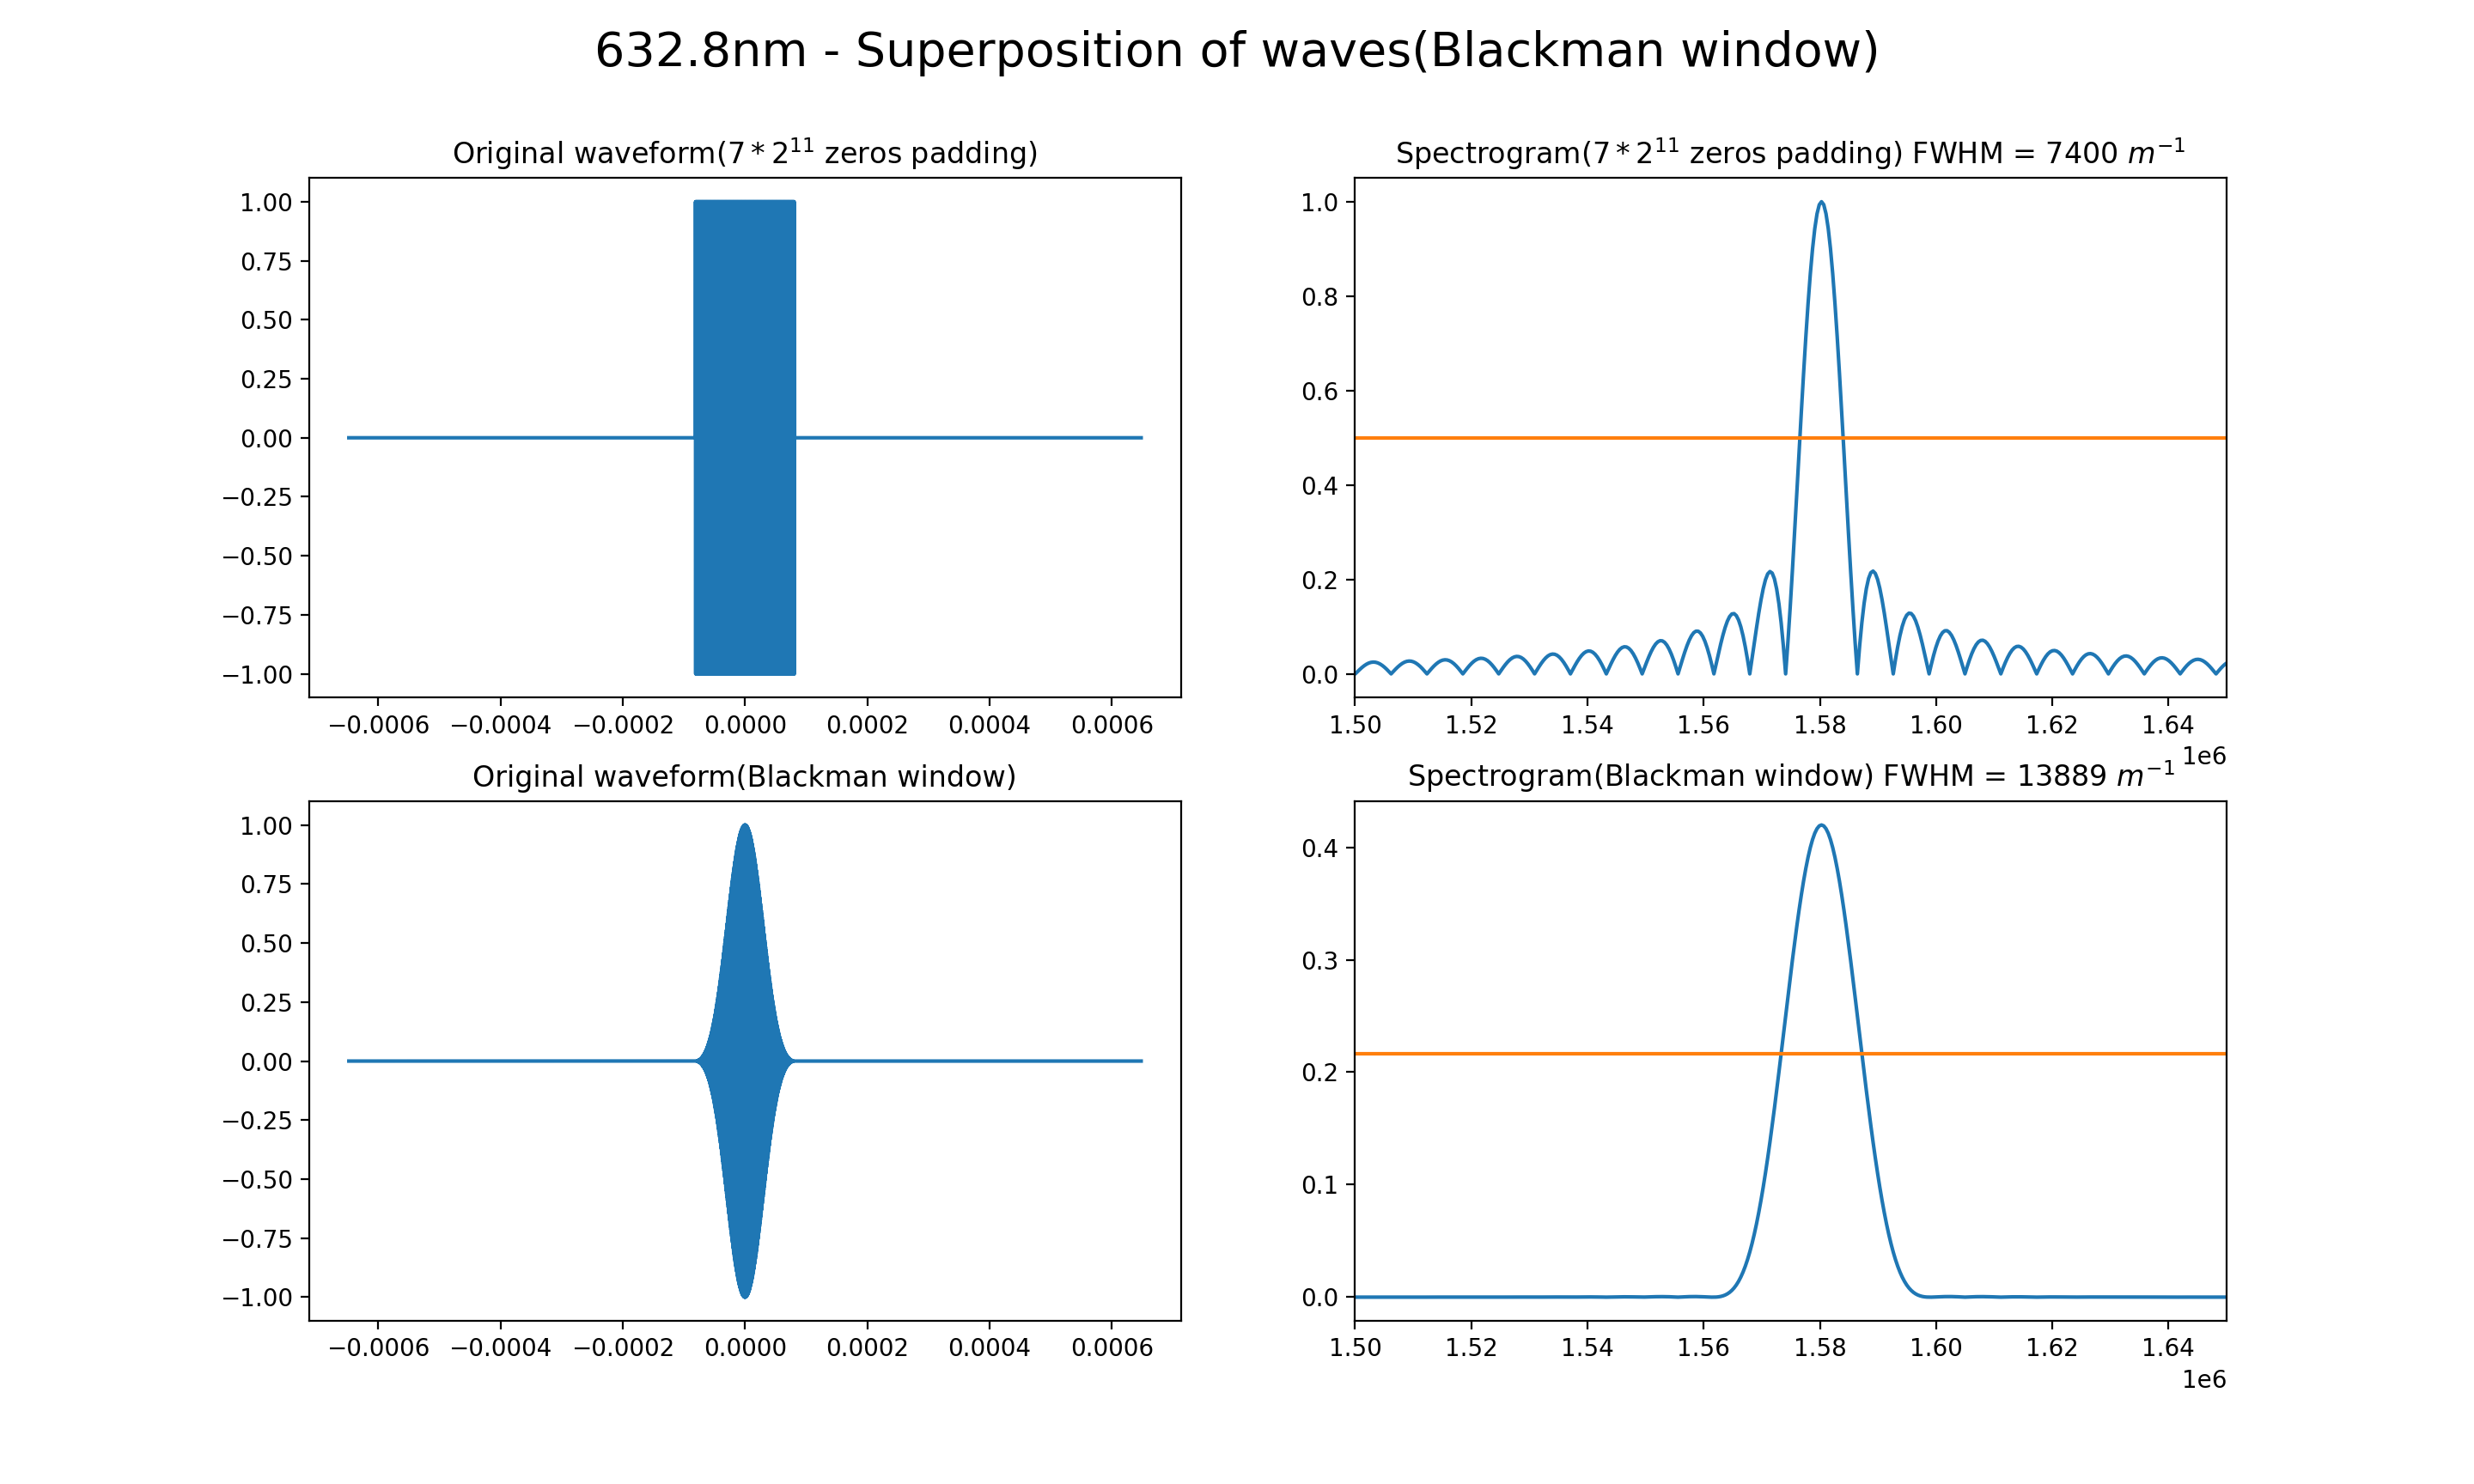
\includegraphics[width=0.5\textwidth]{Blackman.png}}
    \caption{对干涉图分别加Blackman窗与矩形窗的比较,图片左侧显示了干涉图加窗的波形,右侧图片为光谱测量曲线的波形,右侧黄色部分的线表示光谱测量曲线的半波全宽}
    \label{pic14}
\end{figure}

\begin{figure}[htbp]
    \centerline{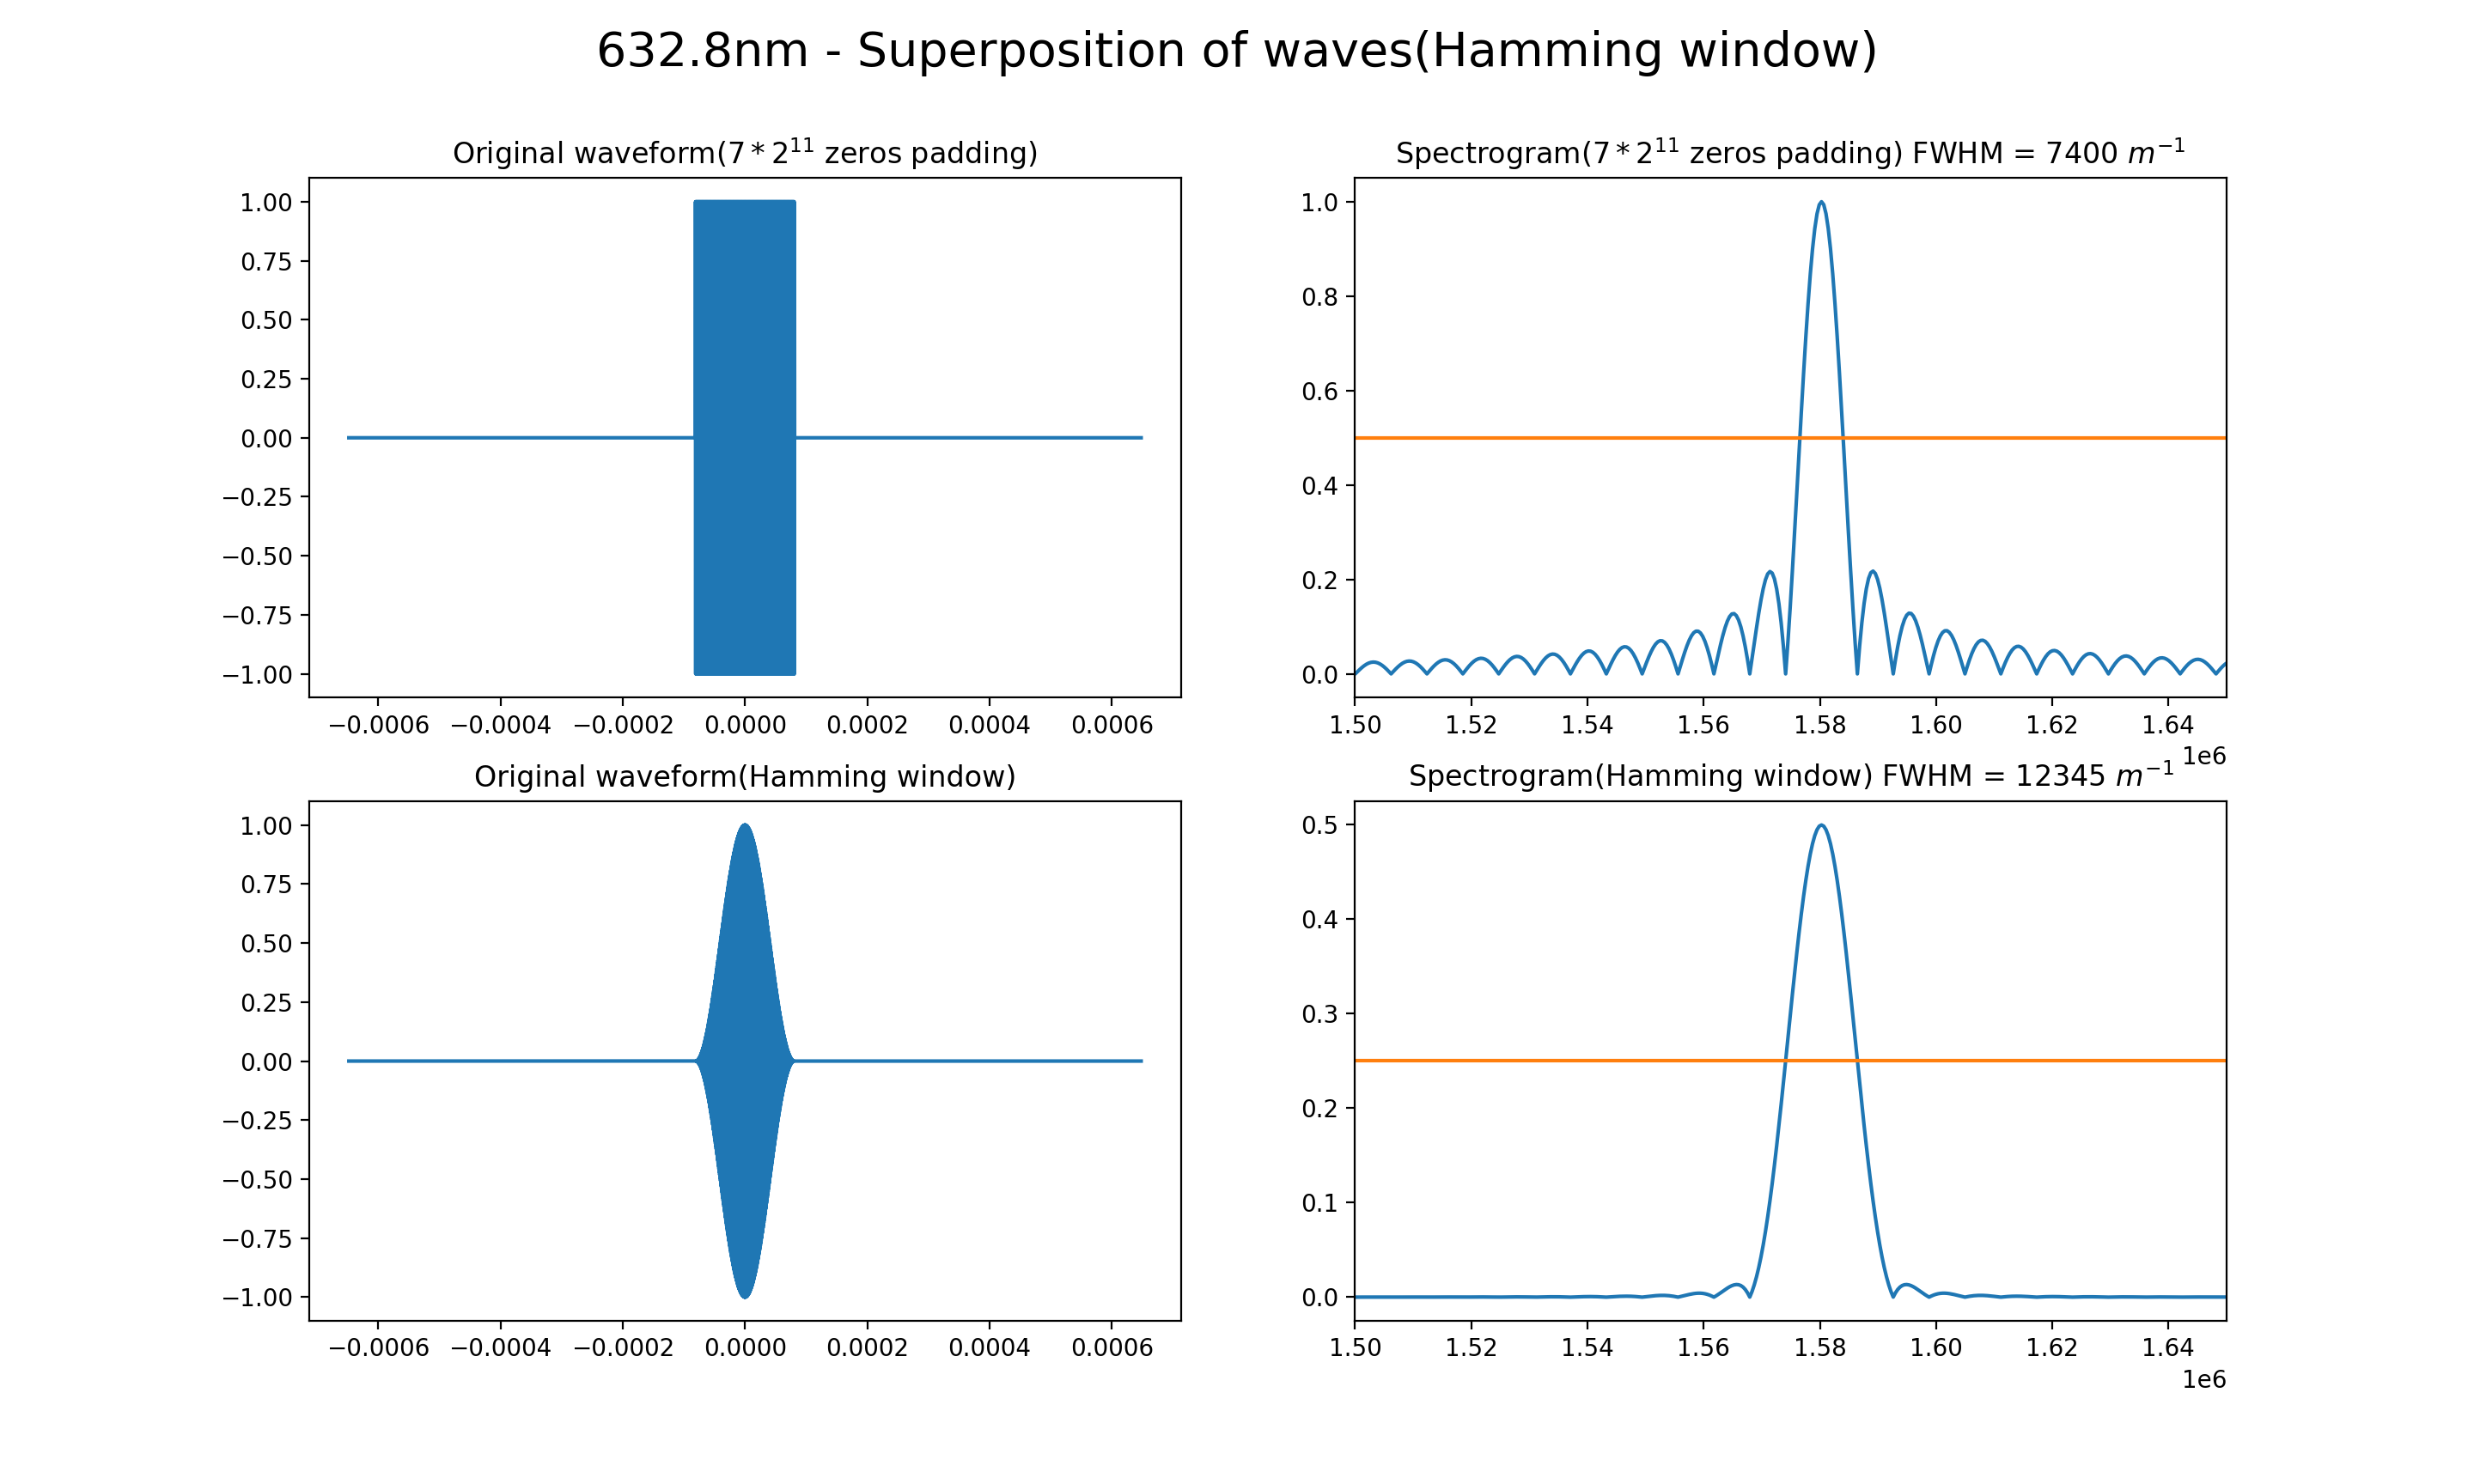
\includegraphics[width=0.5\textwidth]{hamming.png}}
    \caption{对干涉图分别加Hamming窗与矩形窗的比较,图片左侧显示了干涉图加窗的波形,右侧图片为光谱测量曲线的波形,右侧黄色部分的线表示光谱测量曲线的半波全宽}
    \label{pic15}
\end{figure}

\begin{figure}[htbp]
    \centerline{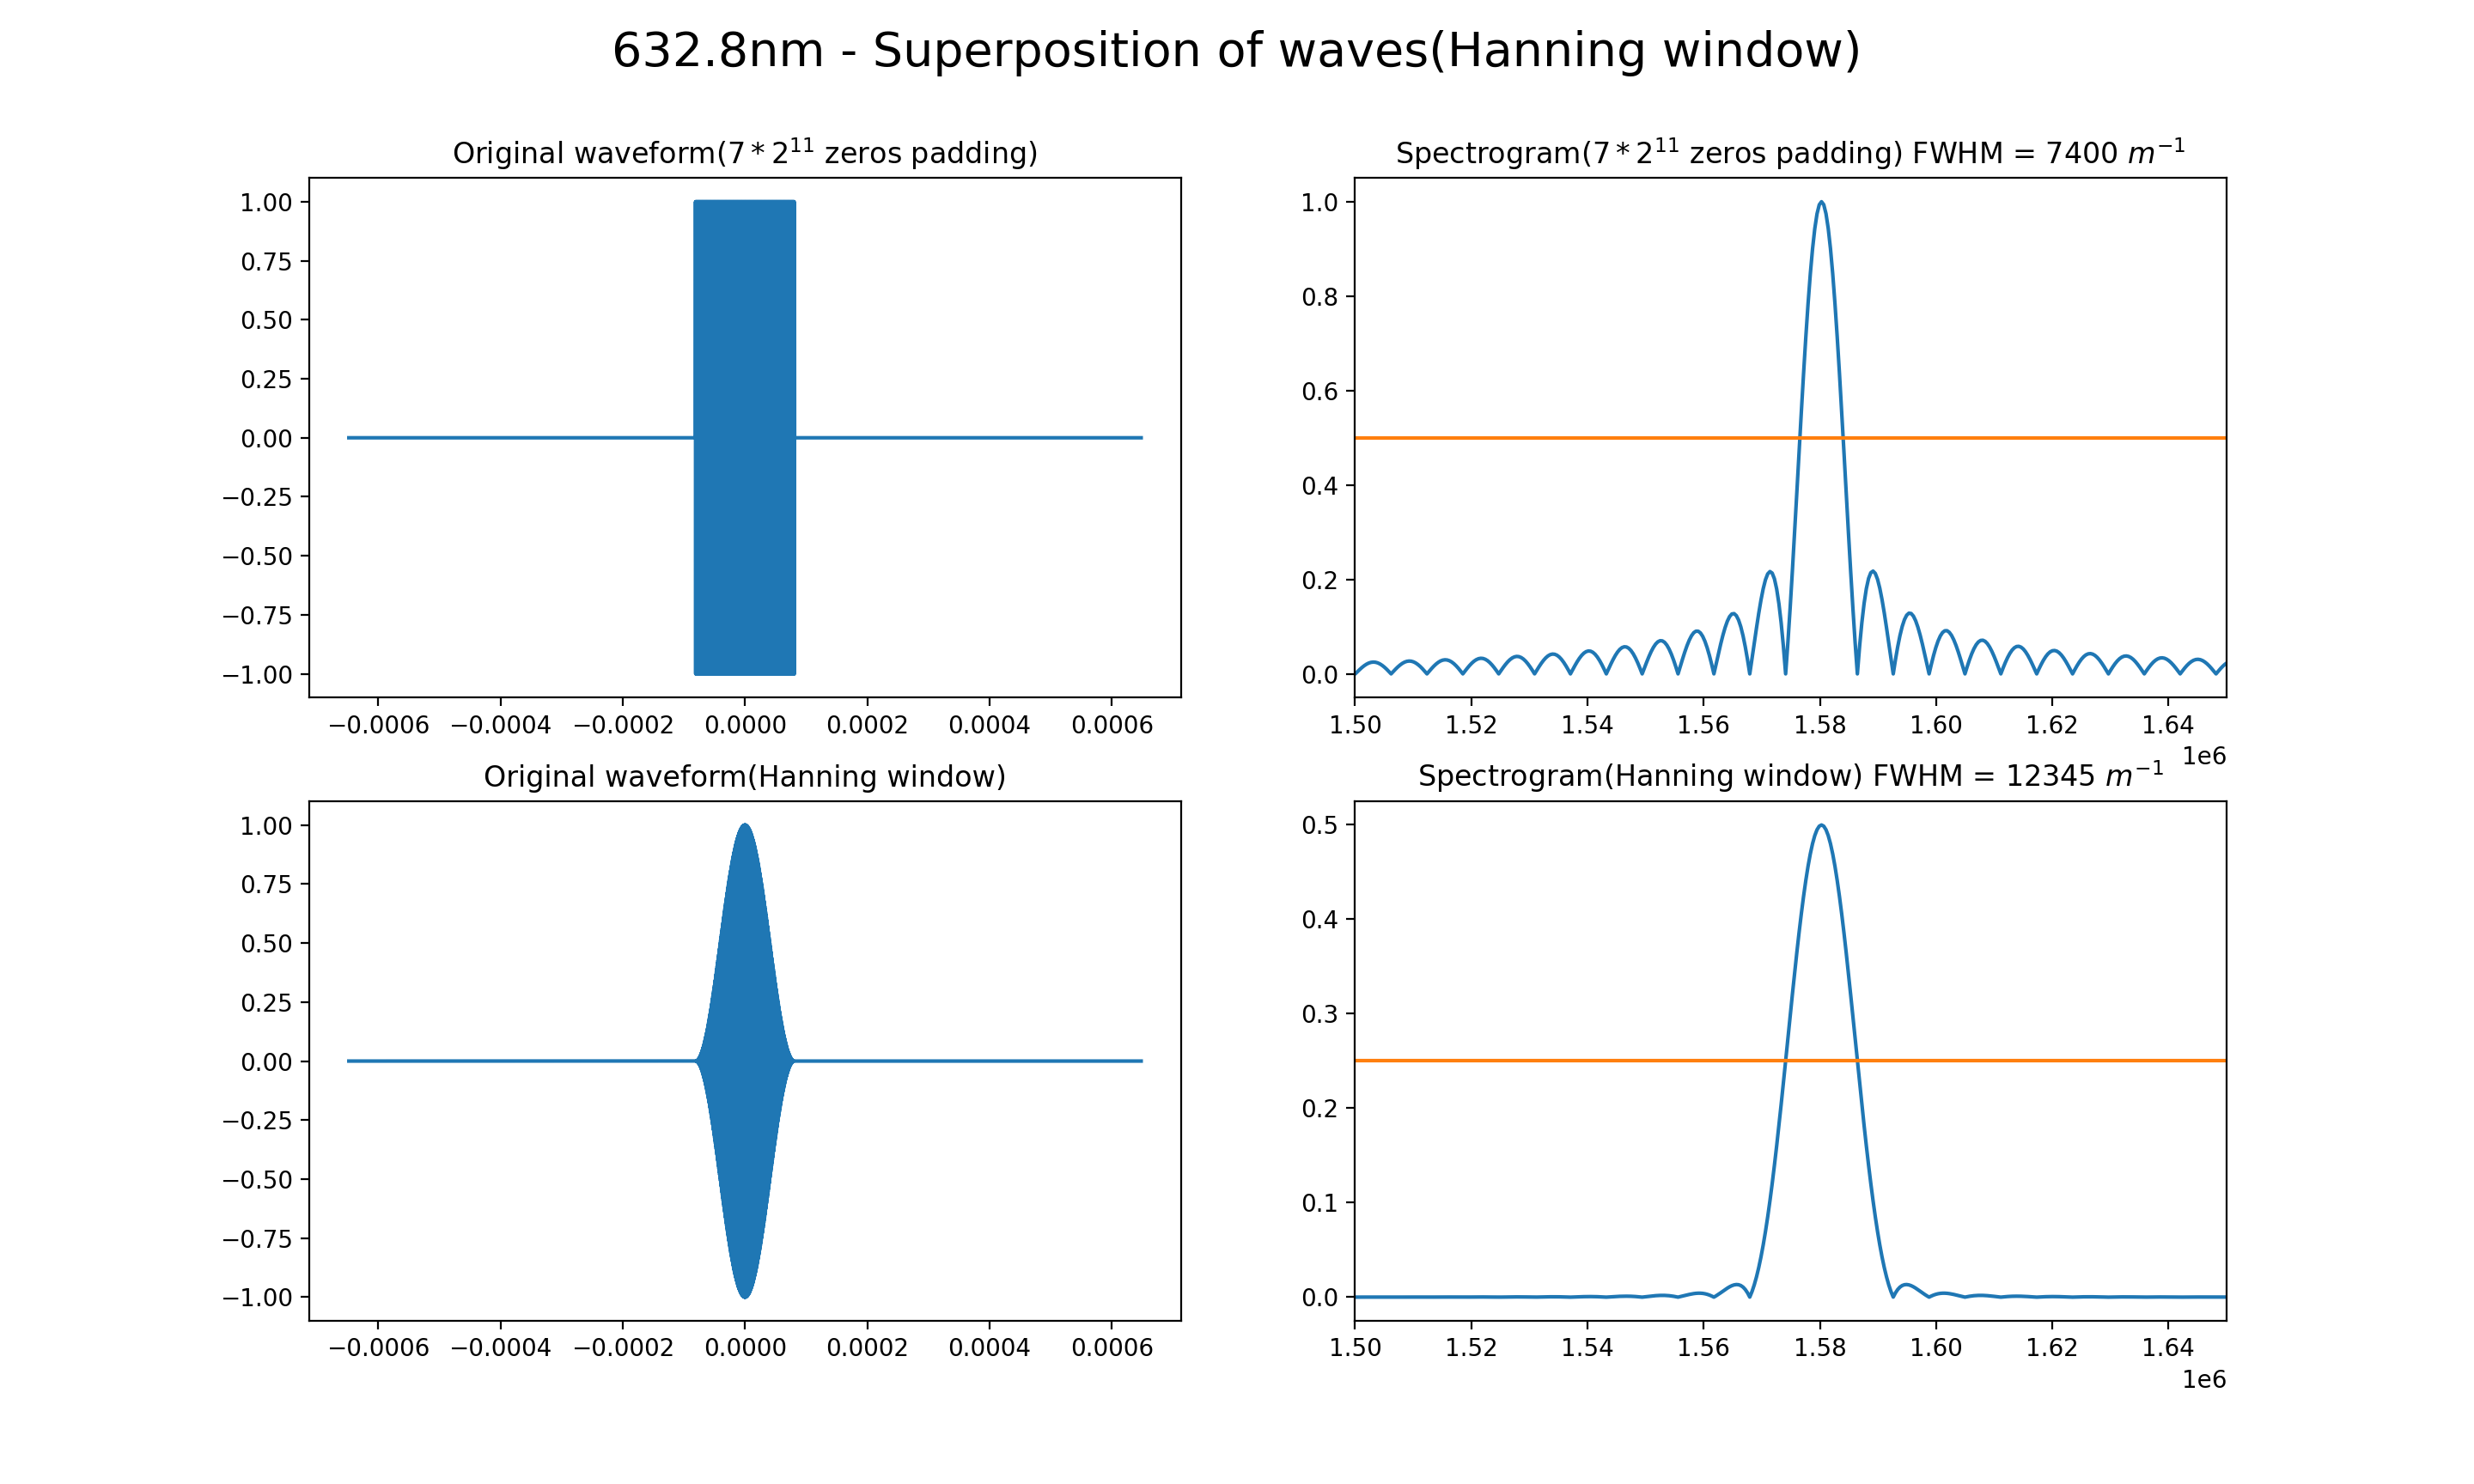
\includegraphics[width=0.5\textwidth]{Hanning.png}}
    \caption{对干涉图分别加Hanning窗与矩形窗的比较,图片左侧显示了干涉图加窗的波形,右侧图片为光谱测量曲线的波形,右侧黄色部分的线表示光谱测量曲线的半波全宽}
    \label{pic16}
\end{figure}

\begin{figure}[htbp]
    \centerline{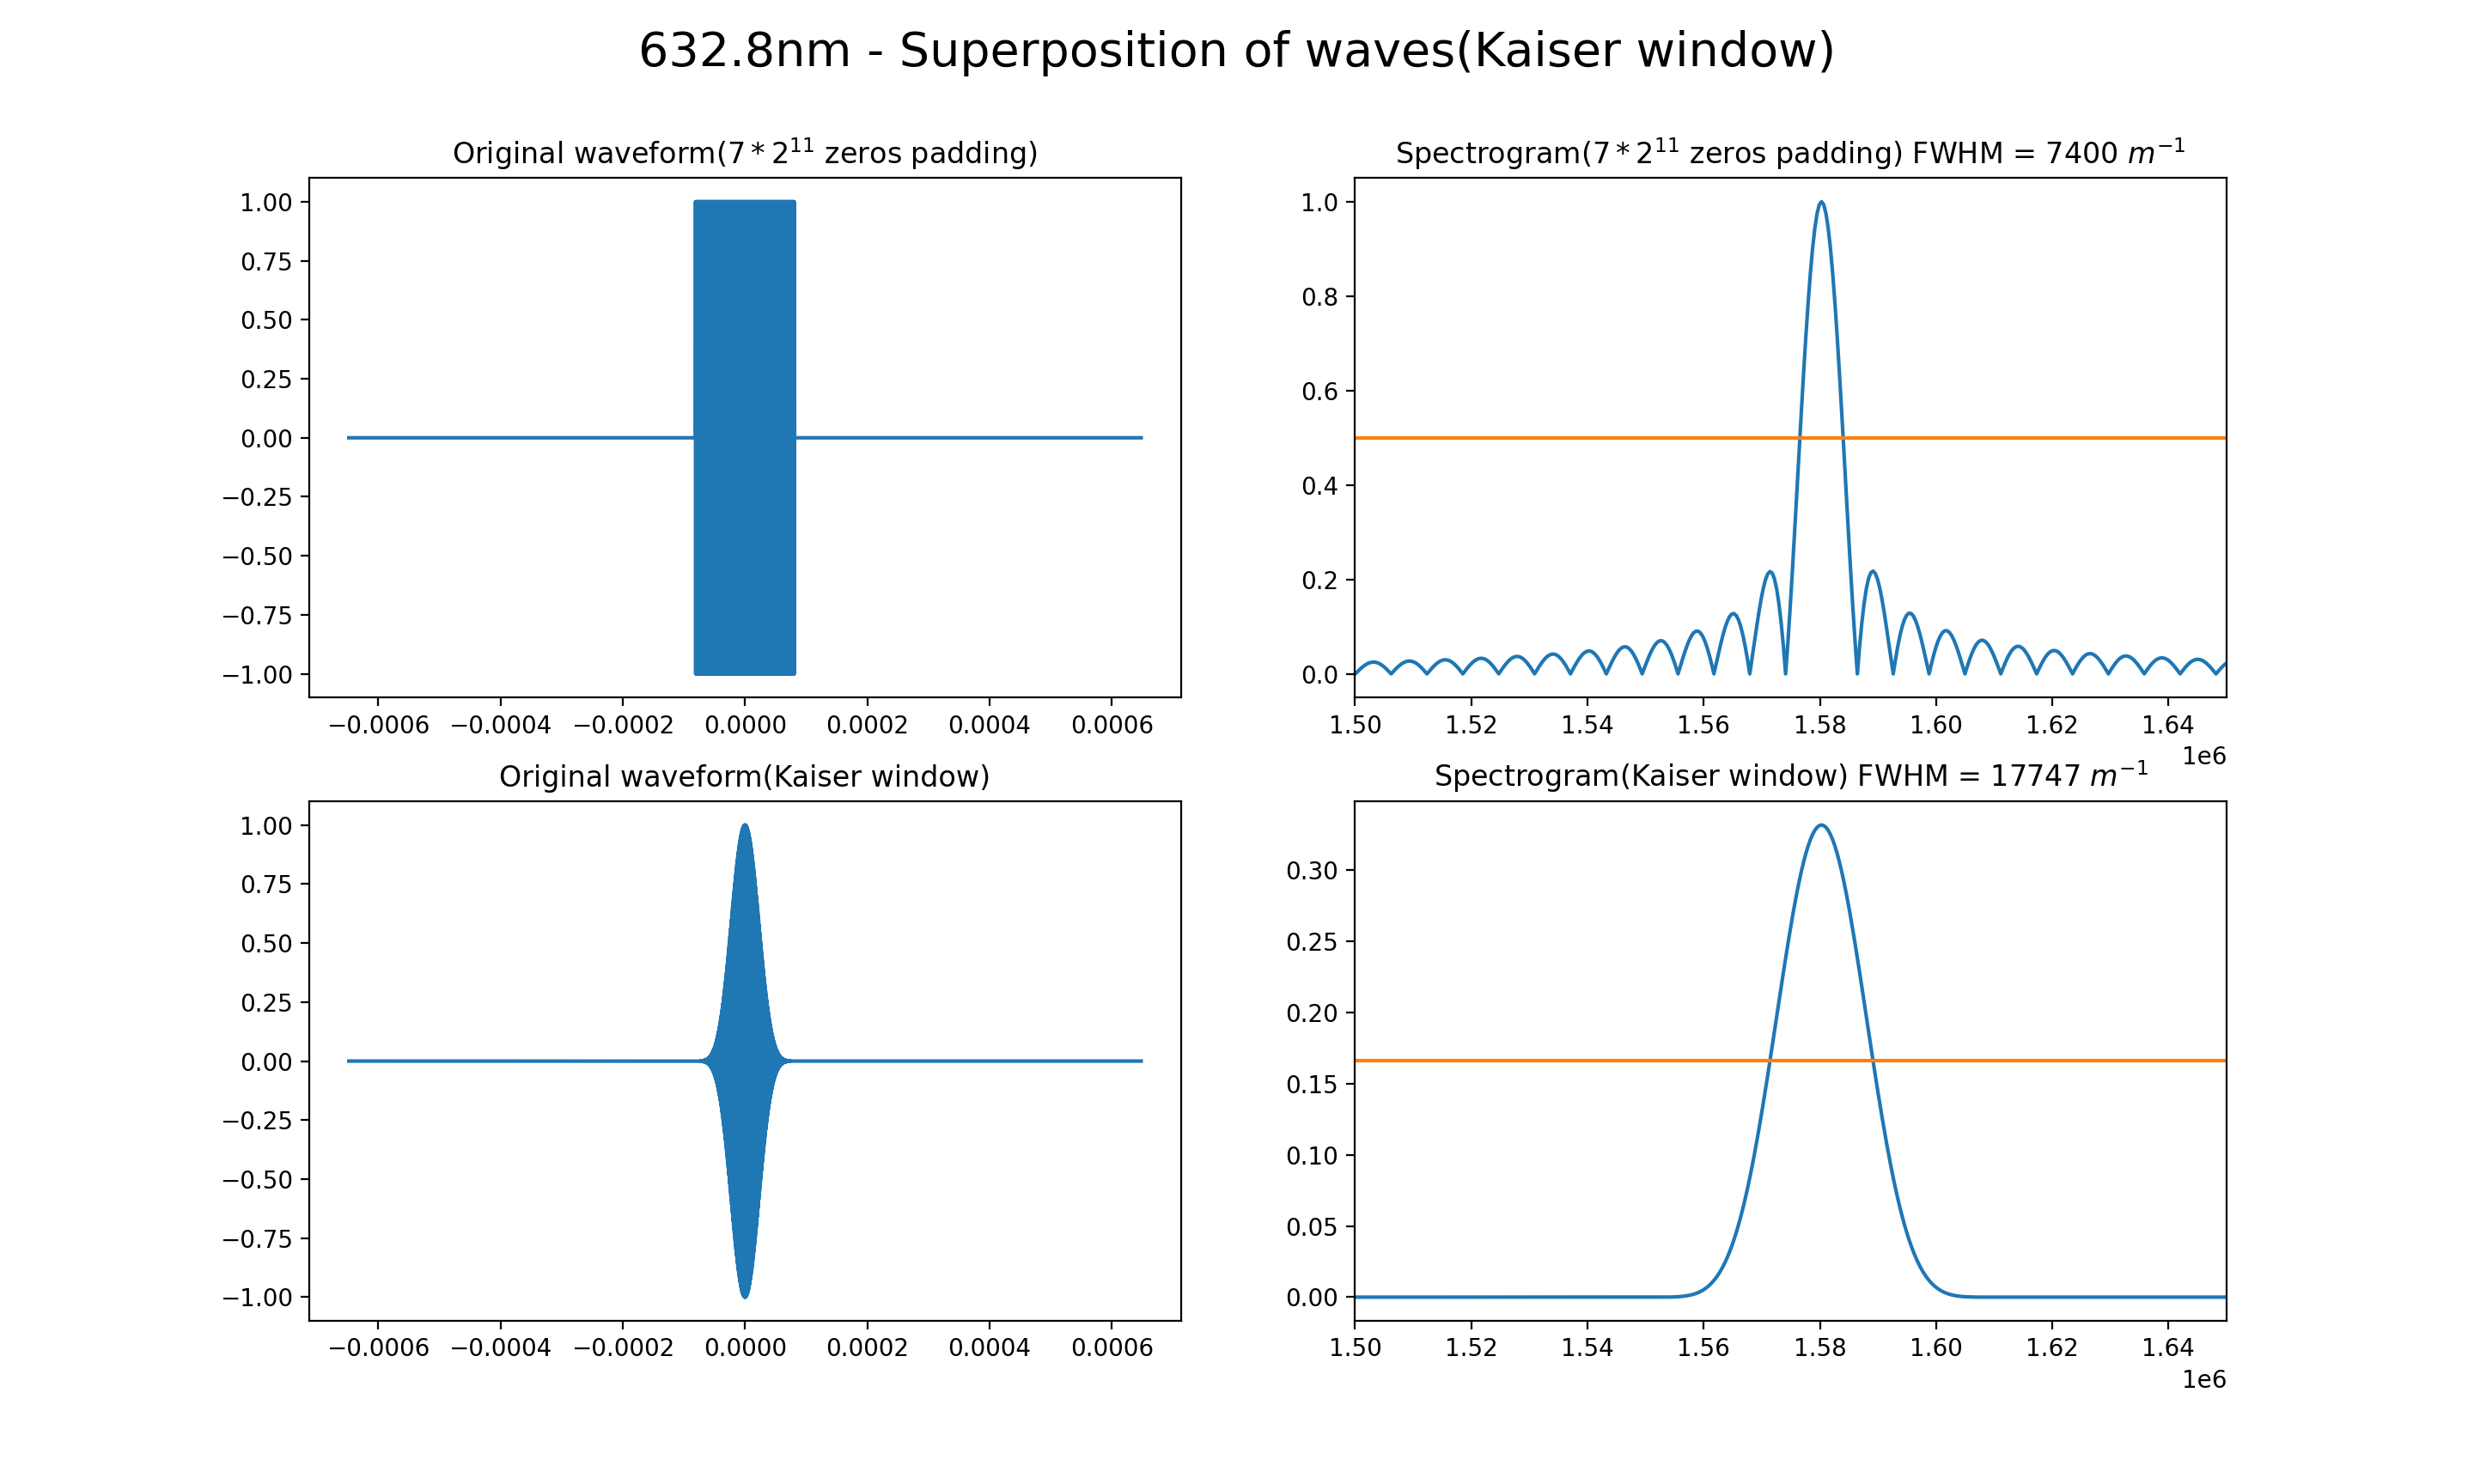
\includegraphics[width=0.5\textwidth]{Kaiser.png}}
    \caption{对干涉图分别加Kaiser窗与矩形窗的比较,图片左侧显示了干涉图加窗的波形,右侧图片为光谱测量曲线的波形,右侧黄色部分的线表示光谱测量曲线的半波全宽}
    \label{pic17}
\end{figure}

图\ref{pic13}至\ref{pic17}表明对干涉图加窗函数后将导致原先光谱测量曲线的幅值部分下降,其中加Kaiser窗对光谱测量曲线的幅值影响最大,但Kaiser窗对光谱测量曲线的边频分量的抑制效果最佳。

对干涉图加窗函数还将导致光谱测量曲线半波全宽变宽的结果。几乎所有窗函数处理后的干涉图的光谱测量曲线的半波宽度均大于使用矩形窗函数(未加窗)处理后的干涉图的光谱测量曲线的半波宽度(图片\ref{pic7}),其中加Kaiser窗对光谱测量曲线的半波宽度影响最大,Hamming窗与Bartlett窗对光谱测量曲线的半波宽度影响较小,但Bartlett窗对光谱测量曲线的边频分量的抑制效果较差。

对干涉图加窗函数的优势在于通过加窗后,干涉图对应的光谱测量曲线的边频分量可以得到有效的抑制。用Kaiser窗处理后的干涉图对应的光谱测量曲线的边频分量的抑制效果最为明显,Balckman窗处理后的效果次之。

\subsection{补零实验结果}
图片\ref{pic1}显示了补$2^{11}$个零与未补零的光谱测量曲线的比较结果。图片\ref{pic2}显示了补$3\times2^{11}$个零与未补零的光谱测量曲线的比较结果。图片\ref{pic3}显示了补$7\times2^{11}$个零与未补零的光谱测量曲线的比较结果。三个图中,黄色的线代表光谱测量曲线的半波全宽。

图\ref{pic1},图\ref{pic2}与图\ref{pic3}显示了对干涉图补零不会影响光谱测量曲线的半波全宽,从频域角度分析,对干涉图补零不会影响频谱的分辨率,补零操作增大了系统的采样点个数,这种操作对FFT分辨率有较好的提升,同时带来了频域波形更加光滑的结果。
\begin{figure}[htbp]
    \centerline{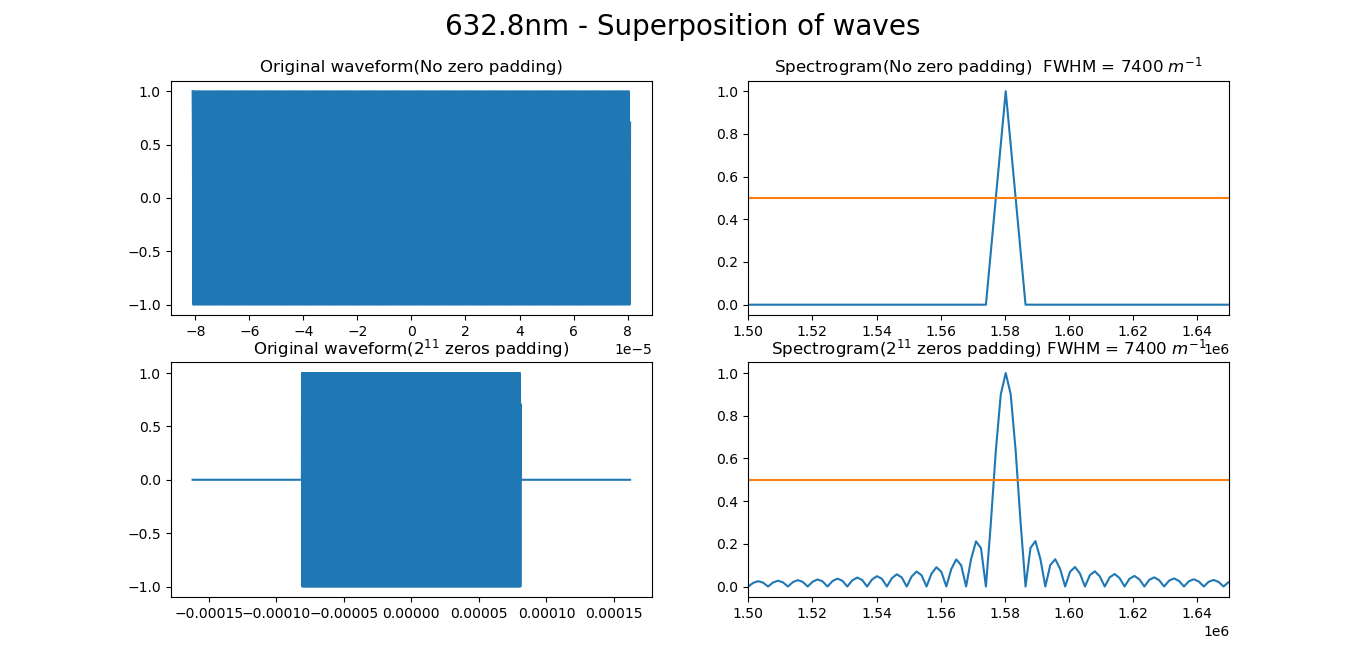
\includegraphics[width=0.5\textwidth]{pic1.png}}
    \caption{补$2^{11}$个零与未补零光谱测量曲线的比较}
    \label{pic1}
\end{figure}

\begin{figure}[htbp]
    \centerline{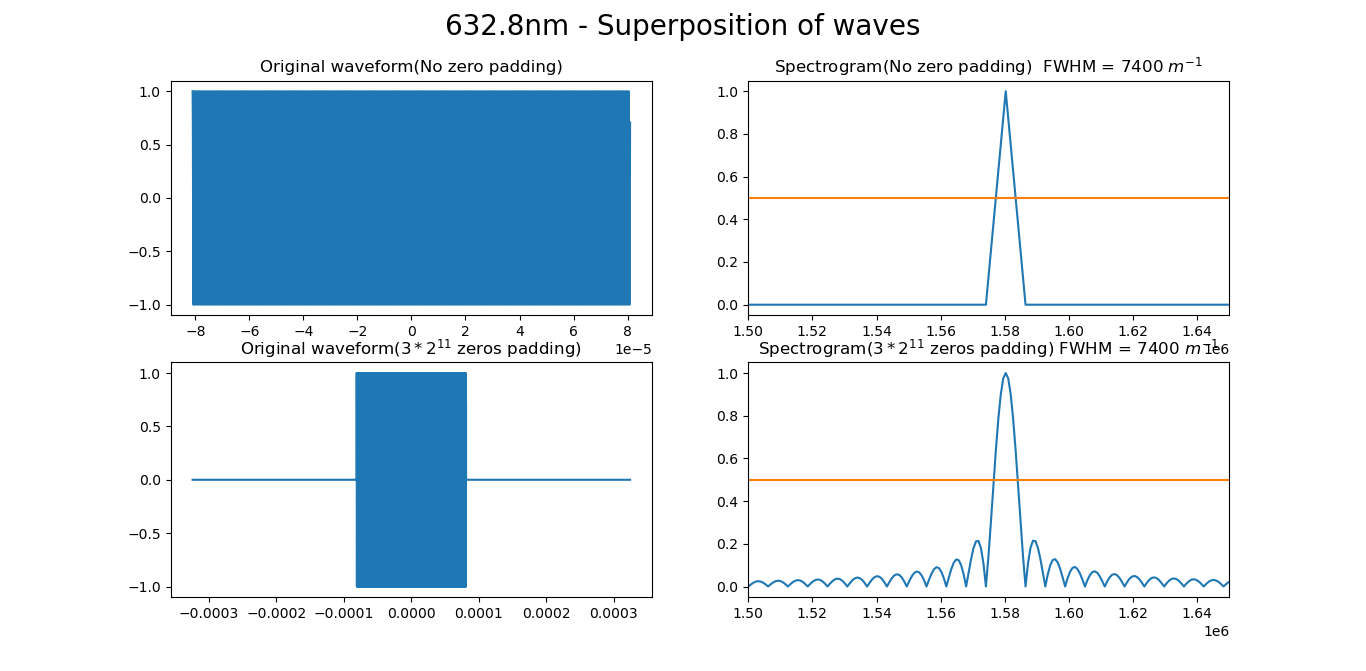
\includegraphics[width=0.5\textwidth]{pic2.png}}
    \caption{补$3\times2^{11}$个零与未补零光谱测量曲线的比较}
    \label{pic2}
\end{figure}

\begin{figure}[htbp]
    \centerline{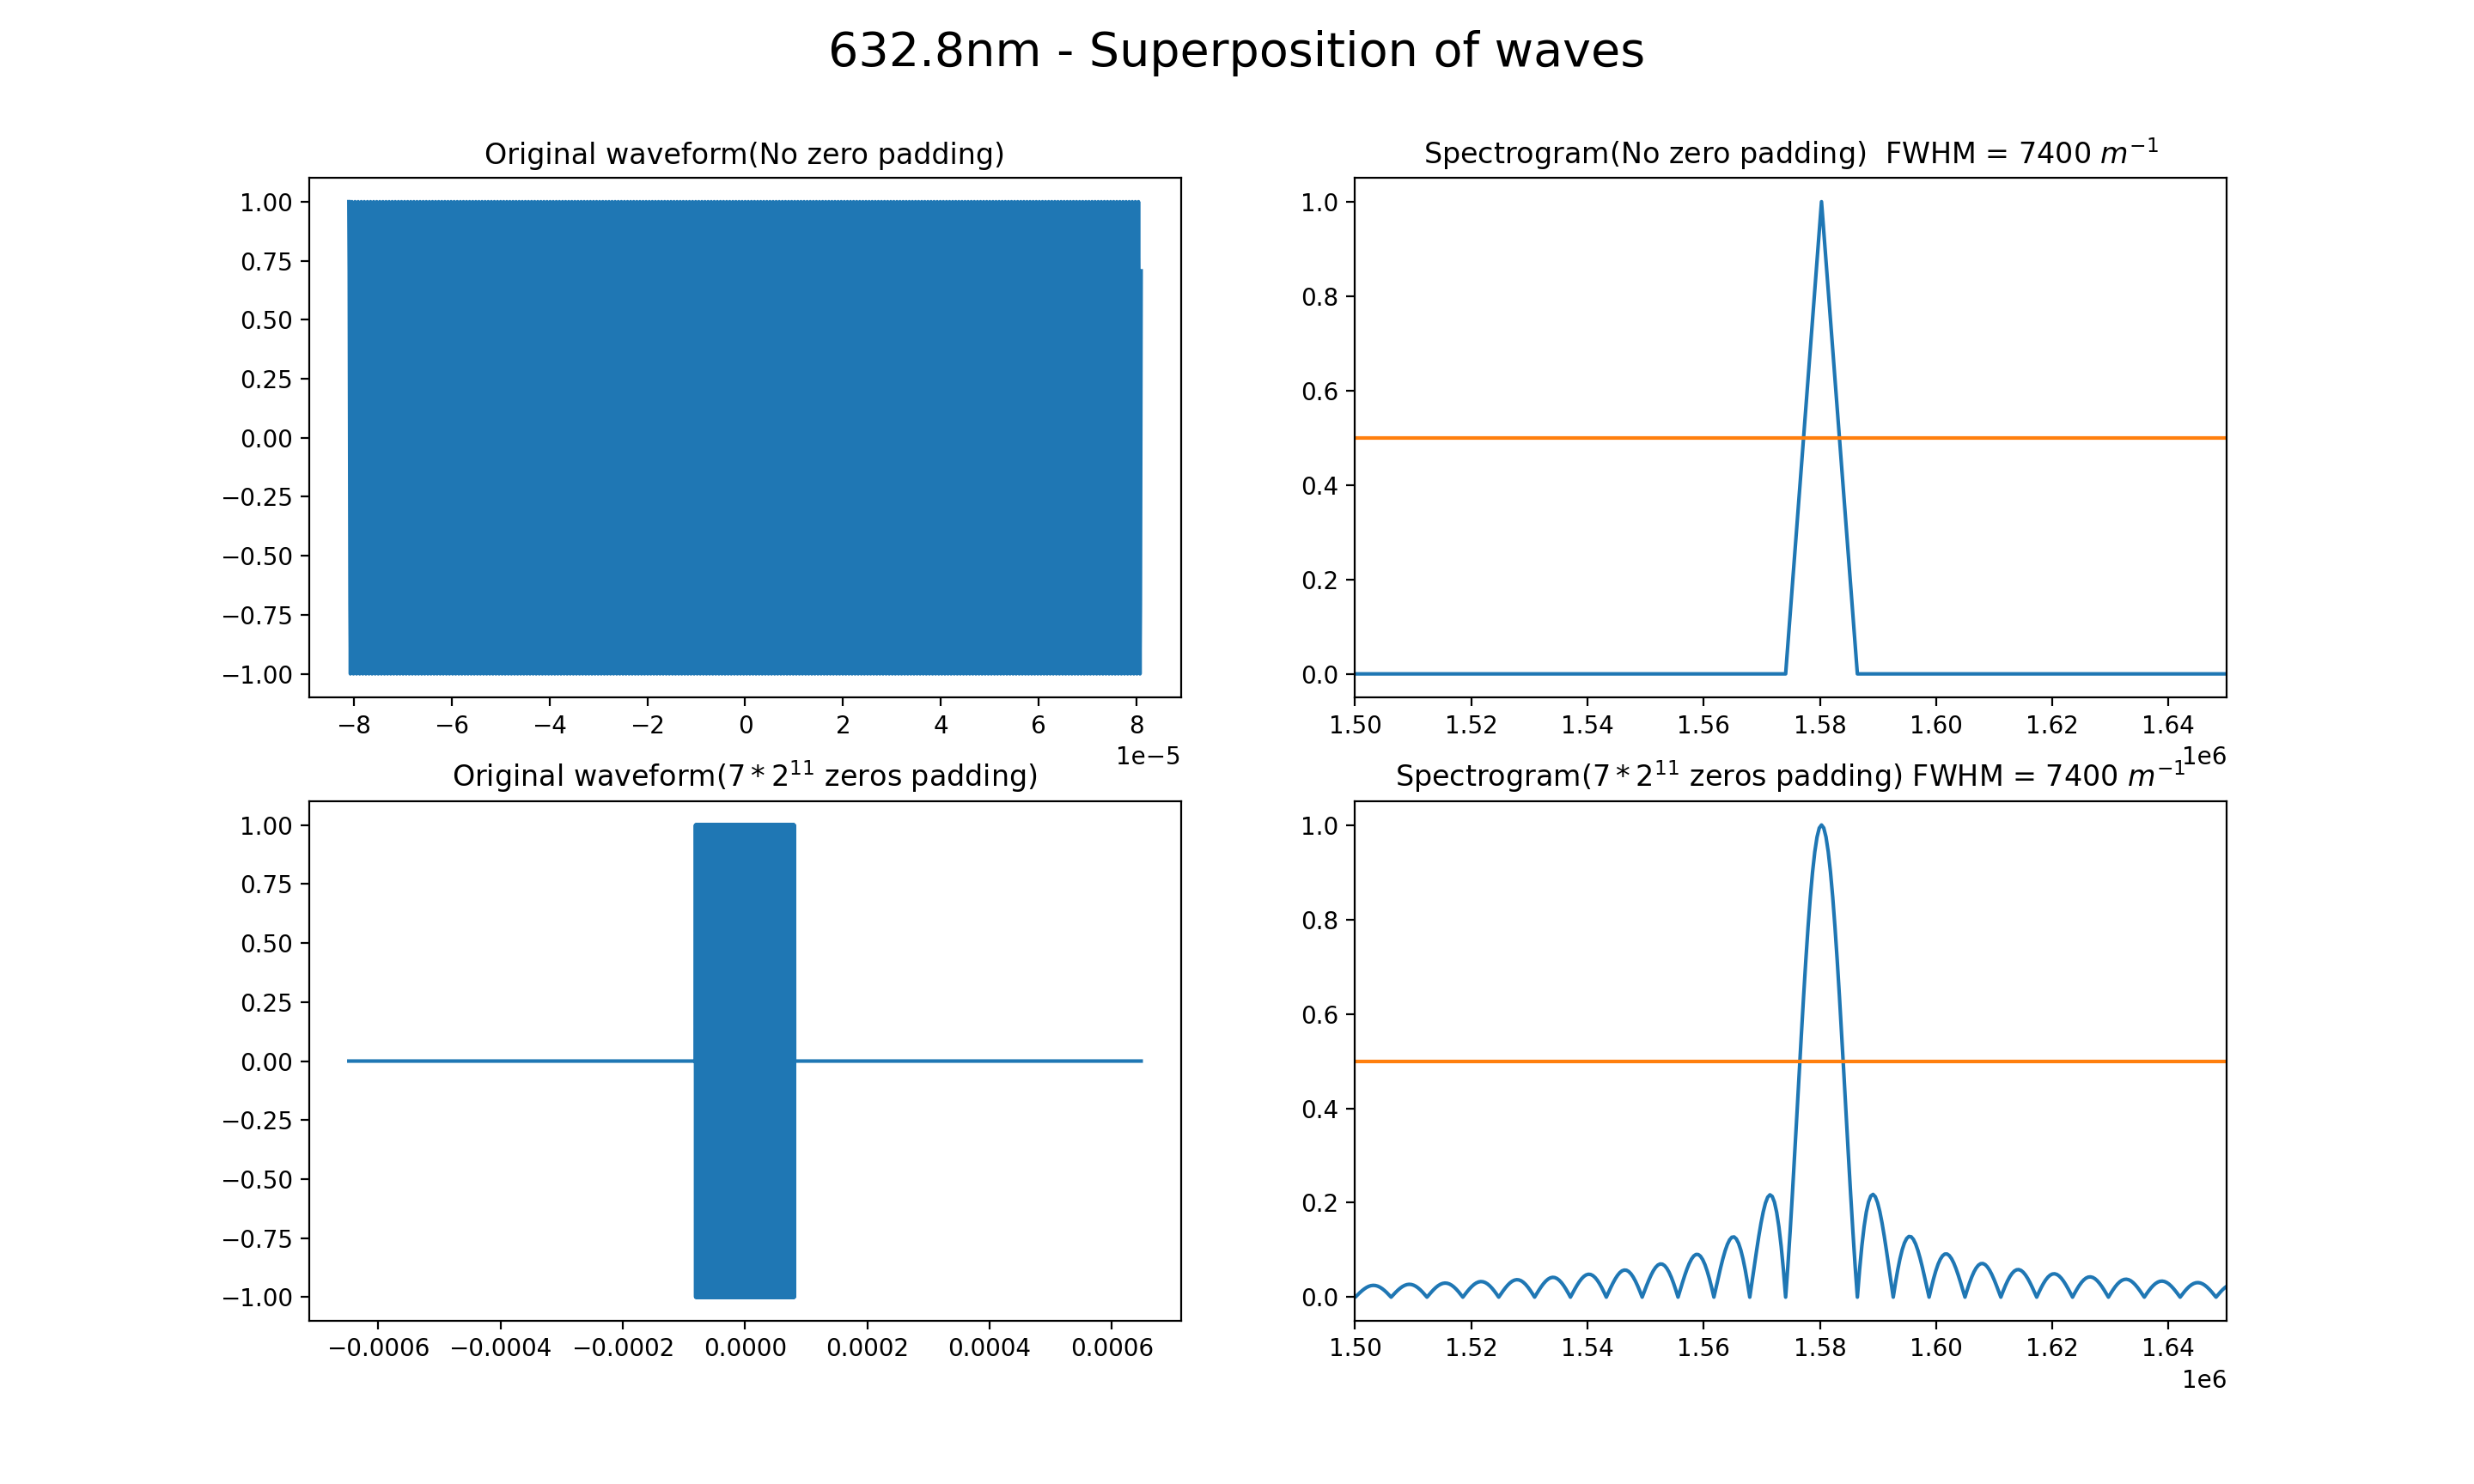
\includegraphics[width=0.5\textwidth]{pic3.png}}
    \caption{补$7\times2^{11}$个零与未补零光谱测量曲线的比较}
    \label{pic3}
\end{figure}

\subsection{仿真结论}
通过上述对仿真结果的讨论,可以得到如下结论:
\begin{itemize}
    \item[1)] 补0不会影响分辨率,但会使旁瓣增大。
    \item[2)] 补0的数量越多,波形越圆润。
    \item[3)] 加窗可以有效减小旁瓣,但会使分辨率降低。
\end{itemize}



\section{结语}
本实验完成了利用Python分别仿真对干涉图补零与对干涉图加窗两因素影响下的傅里叶变换光谱测量系统的光谱测量曲线的实验。

\appendix[实验代码]
\begin{lstlisting}
import numpy as np
import matplotlib.pyplot as plt
from scipy.fftpack import fft, ifft
from matplotlib.pylab import mpl
from pylab import *
from scipy import signal


def find_best_I_average_value(array, average):
    best_I_average_value = 0
    min_dif = 1
    for i in array:
        if abs(i-average) < min_dif:
            min_dif = abs(i-average)
            best_I_average_value = i

    return best_I_average_value

def find_index(array1, array2):
    first_index = 0
    last_index = 0
    current_index = 0
    for i, j in zip(array1,array2):
        if i < j:
            first_index = current_index
            break
        current_index = current_index + 1
    array2 = array2[::-1]
    array1 = array1[::-1]
    current_index = 0
    for i, j in zip(array1,array2):
        if i < j:
            last_index = current_index
            break
        current_index = current_index + 1
    print("array1.size - last_index - first_index = %d" %(array1.size - last_index - first_index))
    return first_index, array1.size - last_index

# 设置中心波长为632.8nm
laimda0 = 632.8*10**(-9) 
#用79.1nm的采样间隔
i = 79.1*10**(-9) 
# 设置中心点的采样频率
sigma0 = 1/laimda0  

p1 = (-1)*(2**10)*79.1*10**(-9)
p2 = (2**10)*79.1*10**(-9)
p3 = (2**11)
p4 = 2**10

#################################
# 设置干涉图的采样点
#(无补零的情况)
#################################
x0 = np.arange(p1, p2, i)
# 计算采样点的个数 
print("没有补零前x0的长度为 %d" %len(x0))      
# 做傅里叶的点数,取下一个2的次幂
# n0 = 2**(int(np.log2(len(x0)))+1)
n0 = len(x0)
print("n0 length = %d" %n0)
# 干涉图函数
I0=(np.cos(2*np.pi*sigma0*x0))
print("没有补零前I0的长度为 %d" %len(I0)) 

# 这里对I0做n0个点的FFT,为了求得正确的幅度需要除以len(x0)
# 真实的点个数,不是除以傅立叶变换的点数
Y0 = 2*abs(fft(I0,n0))/len(x0)
# 得到的Y0是周期函数,为了使用 FWHM函数需要提取出前一半图像
Y0 = Y0[:int(n0/2)]

# 设置频谱图的横坐标
fs = 1/i*np.arange(n0/2)/n0

best_Y0_average_range = 0.5*np.ones((Y0.size, 1))

###############################
# Zero padding begins here
# Case 1.
#   1*2^11 zeros
################################
zero_numbers_1= p3/2
x1 = np.arange((-1)*(p4+zero_numbers_1)*i, (p4+zero_numbers_1)*i, i)
print("补零后x1的长度为 %d" %len(x1)) 
# 做傅里叶的点数,取下一个2的次幂
n1 = 2**(int(np.log2(len(x1)))+1)
print("n1 length = %d" %n1)
I1=(np.cos(2*np.pi*sigma0*x0));

I1 = np.pad(I1,(0,int(zero_numbers_1)),'constant',constant_values = (0,0))
I1 = np.pad(I1,(int(zero_numbers_1),0),'constant',constant_values = (0,0))
print("补零后I1的长度为 %d" %len(I1)) 


Y1 = 2*abs(fft(I1,n1))/len(x0)
Y1 = Y1[:int(n1/2)]


# 设置频谱图的横坐标
fs_1 = 1/i*np.arange(n1/2)/n1

best_Y1_average_range = 0.5*np.ones((Y1.size, 1))

figure(1)
subplot(2,2,1)
plt.plot(x0, I0)
plt.title("Original waveform(No zero padding)")

subplot(2,2,2)
plt.plot(fs, Y0)
plt.plot(fs,best_Y0_average_range)
plt.title("Spectrogram(No zero padding)  FWHM = 7400 $m^{-1}$")
plt.xlim(1.50*(10**6), 1.65*(10**6))

subplot(2,2,3)
plt.plot(x1, I1)
plt.title("Original waveform($2^{11}$ zeros padding)")

subplot(2,2,4)
plt.plot(fs_1, Y1)
plt.plot(fs_1,best_Y1_average_range)
plt.title("Spectrogram($2^{11}$ zeros padding) FWHM = 7400 $m^{-1}$")
plt.xlim(1.50*(10**6), 1.65*(10**6))

plt.suptitle("632.8nm - Superposition of waves", fontsize = 20)

############################
# Zero padding case 2.
#   3*2^11 zeros
############################
zero_numbers_2= 3*p3/2
x2 = np.arange((-1)*(p4+zero_numbers_2)*i, (p4+zero_numbers_2)*i, i)
print("补零后x1的长度为 %d" %len(x1)) 
# 做傅里叶的点数,取下一个2的次幂
n2 = 2**(int(np.log2(len(x2)))+1)
print("n2 length = %d" %n2)
I2=(np.cos(2*np.pi*sigma0*x0));

I2 = np.pad(I2,(0,int(zero_numbers_2)),'constant',constant_values = (0,0))
I2 = np.pad(I2,(int(zero_numbers_2),0),'constant',constant_values = (0,0))
print("补零后I2的长度为 %d" %len(I2)) 


Y2 = 2*abs(fft(I2,n2))/len(x0)
Y2 = Y2[:int(n2/2)]

# 设置频谱图的横坐标
fs_2 = 1/i*np.arange(n2/2)/n2

best_Y2_average_range = 0.5*np.ones((Y2.size, 1))

figure(2)
subplot(2,2,1)
plt.plot(x0, I0)
plt.title("Original waveform(No zero padding)")

subplot(2,2,2)
plt.plot(fs, Y0)
plt.plot(fs,best_Y0_average_range)
plt.title("Spectrogram(No zero padding)  FWHM = 7400 $m^{-1}$")
plt.xlim(1.50*(10**6), 1.65*(10**6))

subplot(2,2,3)
plt.plot(x2, I2)
plt.title("Original waveform($3*2^{11}$ zeros padding)")

subplot(2,2,4)
plt.plot(fs_2, Y2)
plt.plot(fs_2,best_Y2_average_range)
plt.title("Spectrogram($3*2^{11}$ zeros padding) FWHM = 7400 $m^{-1}$")
plt.xlim(1.50*(10**6), 1.65*(10**6))

plt.suptitle("632.8nm - Superposition of waves", fontsize = 20)

#############################
# Zero padding case 3.
#   5*2^11 zeros
#############################
zero_numbers_3= 5*p3/2
x3 = np.arange((-1)*(p4+zero_numbers_3)*i, (p4+zero_numbers_3)*i, i)
print("补零后x1的长度为 %d" %len(x3)) 
# 做傅里叶的点数,取下一个2的次幂
n3 = 2**(int(np.log2(len(x3)))+1)
print("n3 length = %d" %n1)
I3=(np.cos(2*np.pi*sigma0*x0));

I3 = np.pad(I3,(0,int(zero_numbers_3)),'constant',constant_values = (0,0))
I3 = np.pad(I3,(int(zero_numbers_3),0),'constant',constant_values = (0,0))
print("补零后I3的长度为 %d" %len(I3)) 


Y3 = 2*abs(fft(I3,n3))/len(x0)
Y3 = Y3[:int(n3/2)]

# 设置频谱图的横坐标
fs_3 = 1/i*np.arange(n3/2)/n3

best_Y3_average_range = 0.5*np.ones((Y3.size, 1))

figure(3)
subplot(2,2,1)
plt.plot(x0, I0)
plt.title("Original waveform(No zero padding)")

subplot(2,2,2)
plt.plot(fs, Y0)
plt.plot(fs,best_Y0_average_range)
plt.title("Spectrogram(No zero padding)  FWHM = 7400 $m^{-1}$")
plt.xlim(1.50*(10**6), 1.65*(10**6))

subplot(2,2,3)
plt.plot(x3, I3)
plt.title("Original waveform($5*2^{11}$ zeros padding)")

subplot(2,2,4)
plt.plot(fs_3, Y3)
plt.plot(fs_3,best_Y3_average_range)
plt.title("Spectrogram($5*2^{11}$ zeros padding) FWHM = 7400 $m^{-1}$")
plt.xlim(1.50*(10**6), 1.65*(10**6))

plt.suptitle("632.8nm - Superposition of waves", fontsize = 20)

figure(10)
pic1, = plt.plot(fs, Y0)
pic2, = plt.plot(fs_1, Y1)
pic3, = plt.plot(fs_2, Y2)
pic4, = plt.plot(fs_3, Y3)
plt.title("Spectrogram All in One Picture")
plt.xlim(1.50*(10**6), 1.65*(10**6))

plt.legend(handles=[pic1,pic2,pic3,pic4],labels=['No zero padding', '$1*2^{11}$ zeros padding', '$3*2^{11}$ zeros padding', '$5*2^{11}$ zeros padding'], loc='upper right')


plt.suptitle("632.8nm - Superposition of waves", fontsize = 20)


##################################
# Window function begins here
# Case1.
#   - hamming
##################################

zero_numbers_3= 5*p3/2
x3_hamming = np.arange((-1)*(p4+zero_numbers_3)*i, (p4+zero_numbers_3)*i, i)
print("补零后x3的长度为 %d" %len(x3)) 
# 做傅里叶的点数,取下一个2的次幂
n3_hamming = 2**(int(np.log2(len(x3_hamming)))+1)
print("n3 length = %d" %n1)
I3_hamming=(np.cos(2*np.pi*sigma0*x0))
L = len(I3_hamming)

# 定义hamming窗函数
hamming_window = np.hamming(len(I3_hamming))
# 对 x3加窗
I3_hamming = I3_hamming * hamming_window

I3_hamming = np.pad(I3_hamming,(0,int(zero_numbers_3)),'constant',constant_values = (0,0))
I3_hamming = np.pad(I3_hamming,(int(zero_numbers_3),0),'constant',constant_values = (0,0))
print("补零后I3的长度为 %d" %len(I3)) 



Y3_hamming = 2*abs(fft(I3_hamming,n3_hamming))/len(x0)
Y3_hamming = Y3_hamming[:int(n3/2)]

# 设置频谱图的横坐标
fs_3_hamming = 1/i*np.arange(n3_hamming/2)/n3_hamming

Y3_hamming_average = (Y3_hamming.min()+Y3_hamming.max())/2
print("Y3_hamming min = %24e" %Y3_hamming.min())
print("Y3_hamming max = %24e" %Y3_hamming.max())
print("Y3_hamming_average = %24e" %Y3_hamming_average)

best_Y3_hamming_average_value = find_best_I_average_value(Y3_hamming, Y3_hamming_average)
print("best_Y3_hamming_average_value = %24e" %best_Y3_hamming_average_value)

best_Y3_hamming_average_range = best_Y3_hamming_average_value*np.ones((Y3_hamming.size, 1))
# best_Y3_hamming_average_range = 0.5*np.ones((Y3_hamming.size, 1))

first_index, last_index = find_index(best_Y3_hamming_average_range, Y3_hamming)
hamming_FWHM = fs_3_hamming[last_index] - fs_3_hamming[first_index]
print("Hamming FWHM = %d" %int(hamming_FWHM))

figure(4)
subplot(2,2,1)
plt.plot(x3, I3)
plt.title("Original waveform($5*2^{11}$ zeros padding)")

subplot(2,2,2)
plt.plot(fs_3, Y3)
plt.plot(fs_3,best_Y3_average_range)
plt.title("Spectrogram($5*2^{11}$ zeros padding) FWHM = 7400 $m^{-1}$")
plt.xlim(1.50*(10**6), 1.65*(10**6))

plt.suptitle("632.8nm - Superposition of waves(Hamming window)", fontsize = 20)


subplot(2,2,3)
plt.plot(x3_hamming, I3_hamming)
plt.title("Original waveform(Hamming window)")

subplot(2,2,4)
plt.plot(fs_3_hamming, Y3_hamming)
plt.plot(fs_3_hamming,best_Y3_hamming_average_range)
plt.title("Spectrogram(Hamming window) FWHM = %d $m^{-1}$" %int(hamming_FWHM))
plt.xlim(1.50*(10**6), 1.65*(10**6))


#################################
# Window function begins here
# Case2.
#   - kaiser
#################################

zero_numbers_3= 5*p3/2
x3_kaiser = np.arange((-1)*(p4+zero_numbers_3)*i, (p4+zero_numbers_3)*i, i)
print("补零后x3的长度为 %d" %len(x3)) 
# 做傅里叶的点数,取下一个2的次幂
n3_kaiser = 2**(int(np.log2(len(x3_kaiser)))+1)
print("n3 length = %d" %n3_kaiser)
I3_kaiser=(np.cos(2*np.pi*sigma0*x0));
L = len(I3_kaiser)

# 定义kaiser窗函数
kaiser_window = np.kaiser(len(I3_kaiser), 14)

# 对 x3加窗
I3_kaiser = I3_kaiser * kaiser_window

I3_kaiser = np.pad(I3_kaiser,(0,int(zero_numbers_3)),'constant',constant_values = (0,0))
I3_kaiser = np.pad(I3_kaiser,(int(zero_numbers_3),0),'constant',constant_values = (0,0))
print("补零后I3的长度为 %d" %len(I3)) 



Y3_kaiser = 2*abs(fft(I3_kaiser,n3_kaiser))/len(x0)
Y3_kaiser = Y3_kaiser[:int(n3/2)]

# 设置频谱图的横坐标
fs_3_kaiser = 1/i*np.arange(n3_kaiser/2)/n3_kaiser

Y3_kaiser_average = (Y3_kaiser.min()+Y3_kaiser.max())/2
print("Y3_kaiser min = %24e" %Y3_kaiser.min())
print("Y3_kaiser max = %24e" %Y3_kaiser.max())
print("Y3_kaiser_average = %24e" %Y3_kaiser_average)

best_Y3_kaiser_average_value = find_best_I_average_value(Y3_kaiser, Y3_kaiser_average)
print("best_Y3_kaiser_average_value = %24e" %best_Y3_kaiser_average_value)

best_Y3_kaiser_average_range = best_Y3_kaiser_average_value*np.ones((Y3_kaiser.size, 1))
# best_Y3_hamming_average_range = 0.5*np.ones((Y3_hamming.size, 1))

first_index, last_index = find_index(best_Y3_kaiser_average_range, Y3_kaiser)
kaiser_FWHM = fs_3_kaiser[last_index] - fs_3_kaiser[first_index]
print("kaiser FWHM = %d" %int(kaiser_FWHM))

figure(5)
subplot(2,2,1)
plt.plot(x3, I3)
plt.title("Original waveform($5*2^{11}$ zeros padding)")

subplot(2,2,2)
plt.plot(fs_3, Y3)
plt.plot(fs_3,best_Y3_average_range)
plt.title("Spectrogram($5*2^{11}$ zeros padding) FWHM = 7400 $m^{-1}$")
plt.xlim(1.50*(10**6), 1.65*(10**6))

plt.suptitle("632.8nm - Superposition of waves(Kaiser window)", fontsize = 20)


subplot(2,2,3)
plt.plot(x3_kaiser, I3_kaiser)
plt.title("Original waveform(Kaiser window)")

subplot(2,2,4)
plt.plot(fs_3_kaiser, Y3_kaiser)
plt.plot(fs_3_kaiser,best_Y3_kaiser_average_range)
plt.title("Spectrogram(Kaiser window) FWHM = %d $m^{-1}$" %int(kaiser_FWHM))
plt.xlim(1.50*(10**6), 1.65*(10**6))


##################################
# Window function begins here
# Case3.
#   - hanning
##################################

zero_numbers_3= 5*p3/2
x3_hanning = np.arange((-1)*(p4+zero_numbers_3)*i, (p4+zero_numbers_3)*i, i)
print("补零后x3的长度为 %d" %len(x3_hanning)) 
# 做傅里叶的点数,取下一个2的次幂
n3_hanning = 2**(int(np.log2(len(x3_hanning)))+1)
print("n3 length = %d" %n3_hanning)
I3_hanning=(np.cos(2*np.pi*sigma0*x0));
L = len(I3_hanning)

# 定义kaiser窗函数
hanning_window = np.hanning(len(I3_hanning))

# 对 x3加窗
I3_hanning = I3_hanning * hanning_window

I3_hanning = np.pad(I3_hanning,(0,int(zero_numbers_3)),'constant',constant_values = (0,0))
I3_hanning = np.pad(I3_hanning,(int(zero_numbers_3),0),'constant',constant_values = (0,0))
print("补零后I3的长度为 %d" %len(I3_hanning)) 



Y3_hanning = 2*abs(fft(I3_hanning,n3_hanning))/len(x0)
Y3_hanning = Y3_hanning[:int(n3/2)]

# 设置频谱图的横坐标
fs_3_hanning = 1/i*np.arange(n3_hanning/2)/n3_hanning

Y3_hanning_average = (Y3_hanning.min()+Y3_hanning.max())/2
print("Y3_hanning min = %24e" %Y3_hanning.min())
print("Y3_hanning max = %24e" %Y3_hanning.max())
print("Y3_hanning_average = %24e" %Y3_hanning_average)

best_Y3_hanning_average_value = find_best_I_average_value(Y3_hanning, Y3_hanning_average)
print("best_Y3_hanning_average_value = %24e" %best_Y3_hanning_average_value)

best_Y3_hanning_average_range = best_Y3_hanning_average_value*np.ones((Y3_hanning.size, 1))
# best_Y3_hamming_average_range = 0.5*np.ones((Y3_hamming.size, 1))

first_index, last_index = find_index(best_Y3_hanning_average_range, Y3_hanning)
hanning_FWHM = fs_3_hanning[last_index] - fs_3_hanning[first_index]
print("hanning FWHM = %d" %int(hanning_FWHM))

figure(6)
subplot(2,2,1)
plt.plot(x3, I3)
plt.title("Original waveform($5*2^{11}$ zeros padding)")

subplot(2,2,2)
plt.plot(fs_3, Y3)
plt.plot(fs_3,best_Y3_average_range)
plt.title("Spectrogram($5*2^{11}$ zeros padding) FWHM = 7400 $m^{-1}$")
plt.xlim(1.50*(10**6), 1.65*(10**6))

plt.suptitle("632.8nm - Superposition of waves(Hanning window)", fontsize = 20)


subplot(2,2,3)
plt.plot(x3_hanning, I3_hanning)
plt.title("Original waveform(Hanning window)")

subplot(2,2,4)
plt.plot(fs_3_hanning, Y3_hanning)
plt.plot(fs_3_hanning,best_Y3_hanning_average_range)
plt.title("Spectrogram(Hanning window) FWHM = %d $m^{-1}$" %int(hanning_FWHM))
plt.xlim(1.50*(10**6), 1.65*(10**6))


#########################################
# Window function begins here
# Case4.
#   - blackman
#########################################
zero_numbers_3= 5*p3/2
x3_blackman = np.arange((-1)*(p4+zero_numbers_3)*i, (p4+zero_numbers_3)*i, i)
print("补零后x3的长度为 %d" %len(x3)) 
# 做傅里叶的点数,取下一个2的次幂
n3_blackman = 2**(int(np.log2(len(x3_blackman)))+1)
I3_blackman=(np.cos(2*np.pi*sigma0*x0));
L = len(I3_blackman)

# 定义blackman窗函数
blackman_window = np.blackman(len(I3_blackman))
# 对 x3加窗
I3_blackman = I3_blackman * blackman_window

I3_blackman = np.pad(I3_blackman,(0,int(zero_numbers_3)),'constant',constant_values = (0,0))
I3_blackman = np.pad(I3_blackman,(int(zero_numbers_3),0),'constant',constant_values = (0,0))
print("补零后I3的长度为 %d" %len(I3)) 



Y3_blackman = 2*abs(fft(I3_blackman,n3_blackman))/len(x0)
Y3_blackman = Y3_blackman[:int(n3/2)]

# 设置频谱图的横坐标
fs_3_blackman = 1/i*np.arange(n3_blackman/2)/n3_blackman

Y3_blackman_average = (Y3_blackman.min()+Y3_blackman.max())/2
print("Y3_blackman min = %24e" %Y3_blackman.min())
print("Y3_blackman max = %24e" %Y3_blackman.max())
print("Y3_blackman_average = %24e" %Y3_blackman_average)

best_Y3_blackman_average_value = find_best_I_average_value(Y3_blackman, Y3_blackman_average)
print("best_Y3_blackman_average_value = %24e" %best_Y3_blackman_average_value)

best_Y3_blackman_average_range = best_Y3_blackman_average_value*np.ones((Y3_blackman.size, 1))
# best_Y3_blackman_average_range = 0.5*np.ones((Y3_blackman.size, 1))

first_index, last_index = find_index(best_Y3_blackman_average_range, Y3_blackman)
blackman_FWHM = fs_3_blackman[last_index] - fs_3_blackman[first_index]
print("blackman FWHM = %d" %int(blackman_FWHM))

figure(7)
subplot(2,2,1)
plt.plot(x3, I3)
plt.title("Original waveform($5*2^{11}$ zeros padding)")

subplot(2,2,2)
plt.plot(fs_3, Y3)
plt.plot(fs_3,best_Y3_average_range)
plt.title("Spectrogram($5*2^{11}$ zeros padding) FWHM = 7400 $m^{-1}$")
plt.xlim(1.50*(10**6), 1.65*(10**6))

plt.suptitle("632.8nm - Superposition of waves(Blackman window)", fontsize = 20)


subplot(2,2,3)
plt.plot(x3_blackman, I3_blackman)
plt.title("Original waveform(Blackman window)")

subplot(2,2,4)
plt.plot(fs_3_blackman, Y3_blackman)
plt.plot(fs_3_blackman,best_Y3_blackman_average_range)
plt.title("Spectrogram(Blackman window) FWHM = %d $m^{-1}$" %int(blackman_FWHM))
plt.xlim(1.50*(10**6), 1.65*(10**6))




#####################################
# Window function begins here
# Case5.
#   - bartlett
#####################################

zero_numbers_3= 5*p3/2
x3_bartlett = np.arange((-1)*(p4+zero_numbers_3)*i, (p4+zero_numbers_3)*i, i)
print("补零后x3的长度为 %d" %len(x3_bartlett)) 
# 做傅里叶的点数,取下一个2的次幂
n3_bartlett = 2**(int(np.log2(len(x3_bartlett)))+1)
print("n3 length = %d" %n3_bartlett)
I3_bartlett=(np.cos(2*np.pi*sigma0*x0));
L = len(I3_bartlett)

# 定义kaiser窗函数
bartlett_window = np.bartlett(len(I3_bartlett))

# 对 x3加窗
I3_bartlett = I3_bartlett * bartlett_window

I3_bartlett = np.pad(I3_bartlett,(0,int(zero_numbers_3)),'constant',constant_values = (0,0))
I3_bartlett = np.pad(I3_bartlett,(int(zero_numbers_3),0),'constant',constant_values = (0,0))
print("补零后I3的长度为 %d" %len(I3_bartlett)) 



Y3_bartlett = 2*abs(fft(I3_bartlett,n3_bartlett))/len(x0)
Y3_bartlett = Y3_bartlett[:int(n3/2)]

# 设置频谱图的横坐标
fs_3_bartlett = 1/i*np.arange(n3_bartlett/2)/n3_bartlett

Y3_bartlett_average = (Y3_bartlett.min()+Y3_bartlett.max())/2
print("Y3_bartlett min = %24e" %Y3_bartlett.min())
print("Y3_bartlett max = %24e" %Y3_bartlett.max())
print("Y3_bartlett_average = %24e" %Y3_bartlett_average)

best_Y3_bartlett_average_value = find_best_I_average_value(Y3_bartlett, Y3_bartlett_average)
print("best_Y3_bartlett_average_value = %24e" %best_Y3_bartlett_average_value)

best_Y3_bartlett_average_range = best_Y3_bartlett_average_value*np.ones((Y3_bartlett.size, 1))
# best_Y3_blackman_average_range = 0.5*np.ones((Y3_blackman.size, 1))

first_index, last_index = find_index(best_Y3_bartlett_average_range, Y3_bartlett)
bartlett_FWHM = fs_3_bartlett[last_index] - fs_3_bartlett[first_index]
print("bartlett FWHM = %d" %int(bartlett_FWHM))

figure(8)
subplot(2,2,1)
plt.plot(x3, I3)
plt.title("Original waveform($5*2^{11}$ zeros padding)")

subplot(2,2,2)
plt.plot(fs_3, Y3)
plt.plot(fs_3,best_Y3_average_range)
plt.title("Spectrogram($5*2^{11}$ zeros padding) FWHM = 7400 $m^{-1}$")
plt.xlim(1.50*(10**6), 1.65*(10**6))

plt.suptitle("632.8nm - Superposition of waves(Bartlett window)", fontsize = 20)


subplot(2,2,3)
plt.plot(x3_bartlett, I3_bartlett)
plt.title("Original waveform(Bartlett window)")

subplot(2,2,4)
plt.plot(fs_3_bartlett, Y3_bartlett)
plt.plot(fs_3_bartlett,best_Y3_bartlett_average_range)
plt.title("Spectrogram(Bartlett window) FWHM = %d $m^{-1}$" %int(bartlett_FWHM))
plt.xlim(1.50*(10**6), 1.65*(10**6))


###################################
# 将所有加窗后波形汇总在一个图里面
###################################
figure(9)
l1, = plt.plot(fs_3, Y3)
l2, = plt.plot(fs_3_hanning, Y3_hanning)
l3, = plt.plot(fs_3_kaiser, Y3_kaiser)
l4, = plt.plot(fs_3_hamming, Y3_hamming)
l5, = plt.plot(fs_3_bartlett, Y3_bartlett)
l6, = plt.plot(fs_3_blackman, Y3_blackman)
plt.xlim(1.50*(10**6), 1.65*(10**6))


plt.legend(handles=[l1,l2,l3,l4,l5,l6],labels=['Rectangular window','Hanning window', 'Kaiser window','Hamming window','Bartlett window','Blackman window'], loc='upper right')

plt.suptitle("632.8nm - Superposition of waves", fontsize = 20)

plt.subplots_adjust(left=0.125,
                    bottom=0.1, 
                    right=0.9, 
                    top=0.9, 
                    wspace=0.2, 
                    hspace=0.35)
plt.show()
\end{lstlisting}

\end{document}
